\documentclass[degree=master,tocarialchapter]{thuthesis}
% 选项
%   degree=[bachelor|master|doctor|postdoctor], % 必选,学位类型
%   language=[chinese|english], % 可选(默认:chinese),论文的主要语言
%   secret,                % 可选(默认:关闭),是否有密级
%   tocarialchapter,       % 可选(默认:关闭),章目录中使用黑体(这项表示同时打开下面两项)
%   tocarialchapterentry,  % 可选(默认:关闭),单独控制章标题在目录中使用黑体
%   tocarialchapterpage,   % 可选(默认:关闭),单独控制章页码在目录中使用黑体

% 所有其它可能用到的包都统一放到这里了,可以根据自己的实际添加或者删除。
\usepackage{thuthesis}

% 定义所有的图片文件在 figures 子目录下
\graphicspath{{figures/}}

% 可以在这里修改配置文件中的定义。导言区可以使用中文。
% \def\myname{薛瑞尼}

\begin{document}

%%% 封面部分
\frontmatter
\thusetup{
  %******************************
  % 注意:
  %   1. 配置里面不要出现空行
  %   2. 不需要的配置信息可以删除
  %******************************
  %
  %=====
  % 秘级
  %=====
  secretlevel={秘密},
  secretyear={10},
  %
  %=========
  % 中文信息
  %=========
  ctitle={基于非监督学习的视觉里程计\\阶段研究报告 v\version},
  cdegree={工学硕士},
  cdepartment={计算机科学与技术系},
  cmajor={计算机科学与技术},
  cauthor={霍江浩},
  csupervisor={宋亦旭},
  ccosupervisor={郭岚}, % 联合指导老师
  % 日期自动使用当前时间,若需指定按如下方式修改:
  % cdate={超新星纪元},
  %
  % 博士后专有部分
  catalognumber     = {分类号},  % 可以留空
  udc               = {UDC},  % 可以留空
  id                = {编号},  % 可以留空: id={},
  cfirstdiscipline  = {计算机科学与技术},  % 流动站(一级学科)名称
  cseconddiscipline = {深度学习},  % 专 业(二级学科)名称
  postdoctordate    = {2019 年 7 月——2019 年 8 月},  % 工作完成日期
  postdocstartdate  = {2019 年 7 月 10 日},  % 研究工作起始时间
  postdocenddate    = {2019 年 8 月 31 日},  % 研究工作期满时间
  %
  %=========
  % 英文信息
  %=========
  etitle={Unsupervised Learning based Visual Odometry Research v\version},
  % 这块比较复杂,需要分情况讨论:
  % 1. 学术型硕士
  %    edegree:必须为Master of Arts或Master of Science(注意大小写)
  %             “哲学、文学、历史学、法学、教育学、艺术学门类,公共管理学科
  %              填写Master of Arts,其它填写Master of Science”
  %    emajor:“获得一级学科授权的学科填写一级学科名称,其它填写二级学科名称”
  % 2. 专业型硕士
  %    edegree:“填写专业学位英文名称全称”
  %    emajor:“工程硕士填写工程领域,其它专业学位不填写此项”
  % 3. 学术型博士
  %    edegree:Doctor of Philosophy(注意大小写)
  %    emajor:“获得一级学科授权的学科填写一级学科名称,其它填写二级学科名称”
  % 4. 专业型博士
  %    edegree:“填写专业学位英文名称全称”
  %    emajor:不填写此项
  edegree={Doctor of Engineering},
  emajor={Computer Science and Technology},
  eauthor={Xue Ruini},
  esupervisor={Professor Zheng Weimin},
  eassosupervisor={Chen Wenguang},
  % 日期自动生成,若需指定按如下方式修改:
  % edate={December, 2005},
  %
  % 关键词用“英文逗号”分割
  ckeywords={SLAM, 非监督学习, 深度学习, 视觉里程计},
  ekeywords={TeX, LaTeX, CJK, template, thesis}
}

% 定义中英文摘要和关键字
\begin{cabstract}

  即时定位建图技术(SLAM)通过特定的传感器完成实时的定位、建图任务,在机器人研究
  领域一直有着重要的地位,是机器人完成复杂任务的基石。传统SLAM算法主要依赖激光雷达
  或者单目双目摄像头,基于滤波或者优化算法完成定位和建图任务。
  
  近些年来,随着深度学习的兴起,SLAM领域的研究前沿开始逐渐使用深度学习方法进行探索,
  同传统算法相比,深度学习方法鲁棒性强、配置简单、代码量小并且易于理解。本文根据领域
  内已有的成果,进一步探索了非监督学习的视觉SLAM技术,提出一种基于单目且有绝对尺度
  的非监督slam网络,具体的分析了该网络的各项技术设计,并且给出了阶段性的实验成果。

\end{cabstract}

% 如果习惯关键字跟在摘要文字后面,可以用直接命令来设置,如下:
% \ckeywords{\TeX, \LaTeX, CJK, 模板, 论文}

\begin{eabstract}
   An abstract of a dissertation is a summary and extraction of research work
   and contributions. Included in an abstract should be description of research
   topic and research objective, brief introduction to methodology and research
   process, and summarization of conclusion and contributions of the
   research. An abstract should be characterized by independence and clarity and
   carry identical information with the dissertation. It should be such that the
   general idea and major contributions of the dissertation are conveyed without
   reading the dissertation.

   An abstract should be concise and to the point. It is a misunderstanding to
   make an abstract an outline of the dissertation and words ``the first
   chapter'', ``the second chapter'' and the like should be avoided in the
   abstract.

   Key words are terms used in a dissertation for indexing, reflecting core
   information of the dissertation. An abstract may contain a maximum of 5 key
   words, with semi-colons used in between to separate one another.
\end{eabstract}

% \ekeywords{\TeX, \LaTeX, CJK, template, thesis}

% 如果使用授权说明扫描页,将可选参数中指定为扫描得到的 PDF 文件名,例如:
% \makecover[scan-auth.pdf]
\makecover

%% 目录
\tableofcontents

%% 符号对照表
%\input{data/denotation}


%%% 正文部分
\mainmatter
% !TeX root = ../main.tex

\chapter{移动操作机器人的国内外现状}
\label{cha:intro}

\section{移动操作机器人概念}
\label{cha:base_comcept}

移动操作机器人(Mobile Manipulator)目前仍然是一个非常宽泛的概念,通常我们认为,典型的移动操作
机器人是由一台机械臂和一个可自由移动的平台组成的,机械臂通过某种方式挂载在平台上\cite{bostelman2016survey}。
近年来,随着科技的飞速发展以及制造业转型的巨大压力,移动操作机器人成为新的研究热点,在学术界及
工业界受到了广泛关注\cite{schneier2015literature}。移动操作机器人已经被广泛的应用到了航天\cite{ambrose2004mobile}、医药、制造\cite{guizzo2011meka}、清洁、服务等多个场景,
在各个领域发挥着重要的作用。但移动操作机器人在性能和功能上还远远没有达到我们期待的水平,相
关研究及工业尝试还需要很长时间的发展。

广义的移动操作机器人除机械臂外,可依赖的平台非常多样,除了常见的轮式底盘、平衡车式底盘外,还可
使用无人机作为移动平台,甚至仿人的双足行走底盘。无人机平台的移动操作机器人有夹爪式、机械臂式等
各种种类,近年来也广泛的
受到各界的关注\cite{ruggiero2018aerial}。相比于无人机或者足式底盘,轮式底盘的移动操作机器人负载更
高,性能更强劲,应用更加广泛,功能更加多样,品种也更加丰富,因此本文主要论述以轮式底盘作为移动
平台的移动操作机器人,并给出相应的控制方法。

\section{移动操作机器人国内外应用现状}
\label{cha:application}

近年来,国内外机器人相关的创业公司层出不穷,移动操作机器人行业也是投资机构聚焦的热点。下面本文
将分别介绍移动操作机器人的两大主要部分:机械臂以及移动底盘的应用历史与现状,随后介绍移动操作机器人
作为整体的应用情况。

机械臂作为主要生产工具在制造业承担作用的历史非常久,机械臂在制造业最早的规模化应用被认为诞生
在汽车制造领域。同其他行业相比,汽车领域产品款式固定,出货量大,规模效应强,这些特性使得基于硬编码
控制的大型高精度机械臂得到广泛应用,如图~\ref{fig:armcar} 展示了工业机械臂在汽车产线上应用
的场景。以汽车工业为代表的自动化机器人应用大部分为高精度工业机械臂,其发展已经有近
半个世纪的历史,自1973年ABB和KUKA将工业机器人推向市场后,这一行业迎来了飞速发展,工业机械臂
的厂商不断增加,款式与性能持续丰富,各种面对细分领域的工业机械臂相继面世,如图~\ref{fig:industry_arms}。

\begin{figure}
\centering
\begin{subfigure}{1.\textwidth}
  \centering
  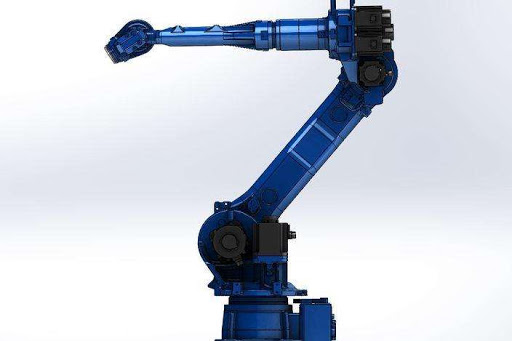
\includegraphics[height=3.5cm]{arm1.jpg}
  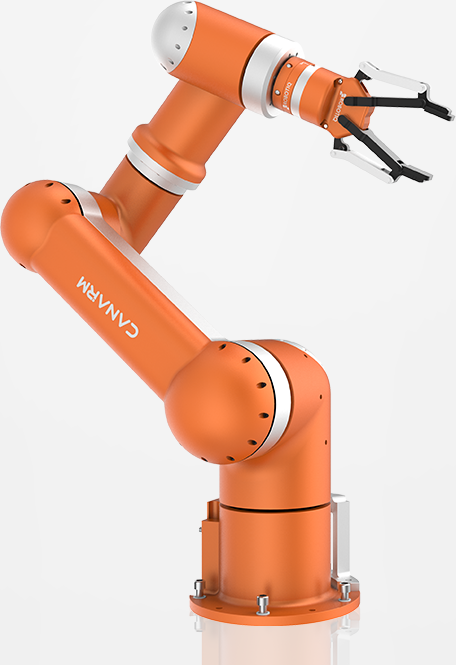
\includegraphics[height=3.5cm]{arm2.png}
  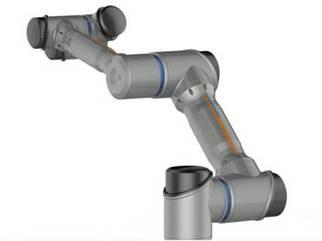
\includegraphics[height=3.5cm]{arm4.jpg}\\
  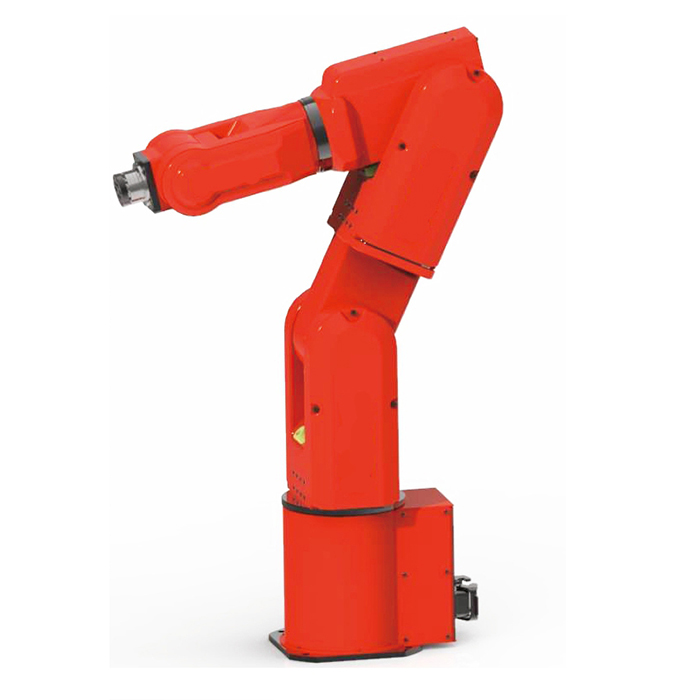
\includegraphics[height=3.5cm]{arm3.jpg}
  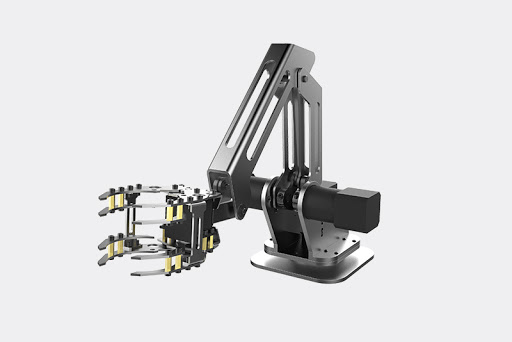
\includegraphics[height=3.5cm]{arm5.jpg}
  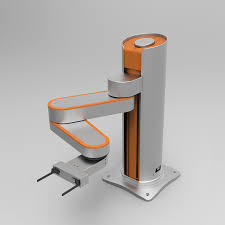
\includegraphics[height=3.5cm]{arm6.jpeg}
\end{subfigure}%
\caption{各式工业机械臂产品}
\label{fig:industry_arms}
\end{figure}


目前,国际
工业机器人领域有四大标杆企业,分别是瑞典 ABB、德国 KUKA、日本FANUC 和日本安川电机。四大厂商
各有所长,ABB擅长控制系统,KUKA优势在于系统集成应用与本体制造,FANUC长于数控系统,安川电机
的优势在于伺服电机制造和运动控制器的研发。除四大头部企业外,美国 Adept Technology、瑞士
Staubli、意大利Comau、日本的川崎、爱普生、那智不二越和中国新松机器人自动化股份有限公司也是
国际工业机器人的重要供应商\cite{huangxihuanReview}。

除汽车工业外,高精度工业机械臂在医疗
领域也取得了不俗的成绩,Intuitive Surgical公司研发的“达芬奇”手术机器人在世界范围内广泛应用,
我国于2006年引入第一套达芬奇手术系统,至今各式手术机器人在中国已累计完成10万例外科手术,如
图~\ref{fig:davinci}。我国华大智造研发的远程
超声检测系统~\ref{fig:huada},该系统在新冠疫情期间的武汉方舱医院内进行了应用测试\cite{wushengzheng20205g},取得了可喜的进展。


\begin{figure}
\centering
\begin{subfigure}{.5\textwidth}
  \centering
  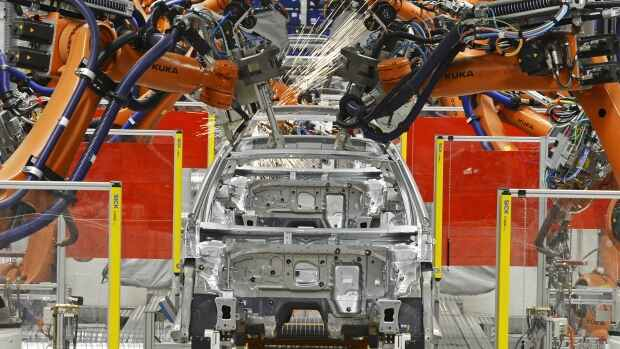
\includegraphics[height=3cm]{kuka_car.jpg}
  \caption{完全由库卡机械臂组成的汽车焊接流水线}
\end{subfigure}%
\begin{subfigure}{.5\textwidth}
  \centering
  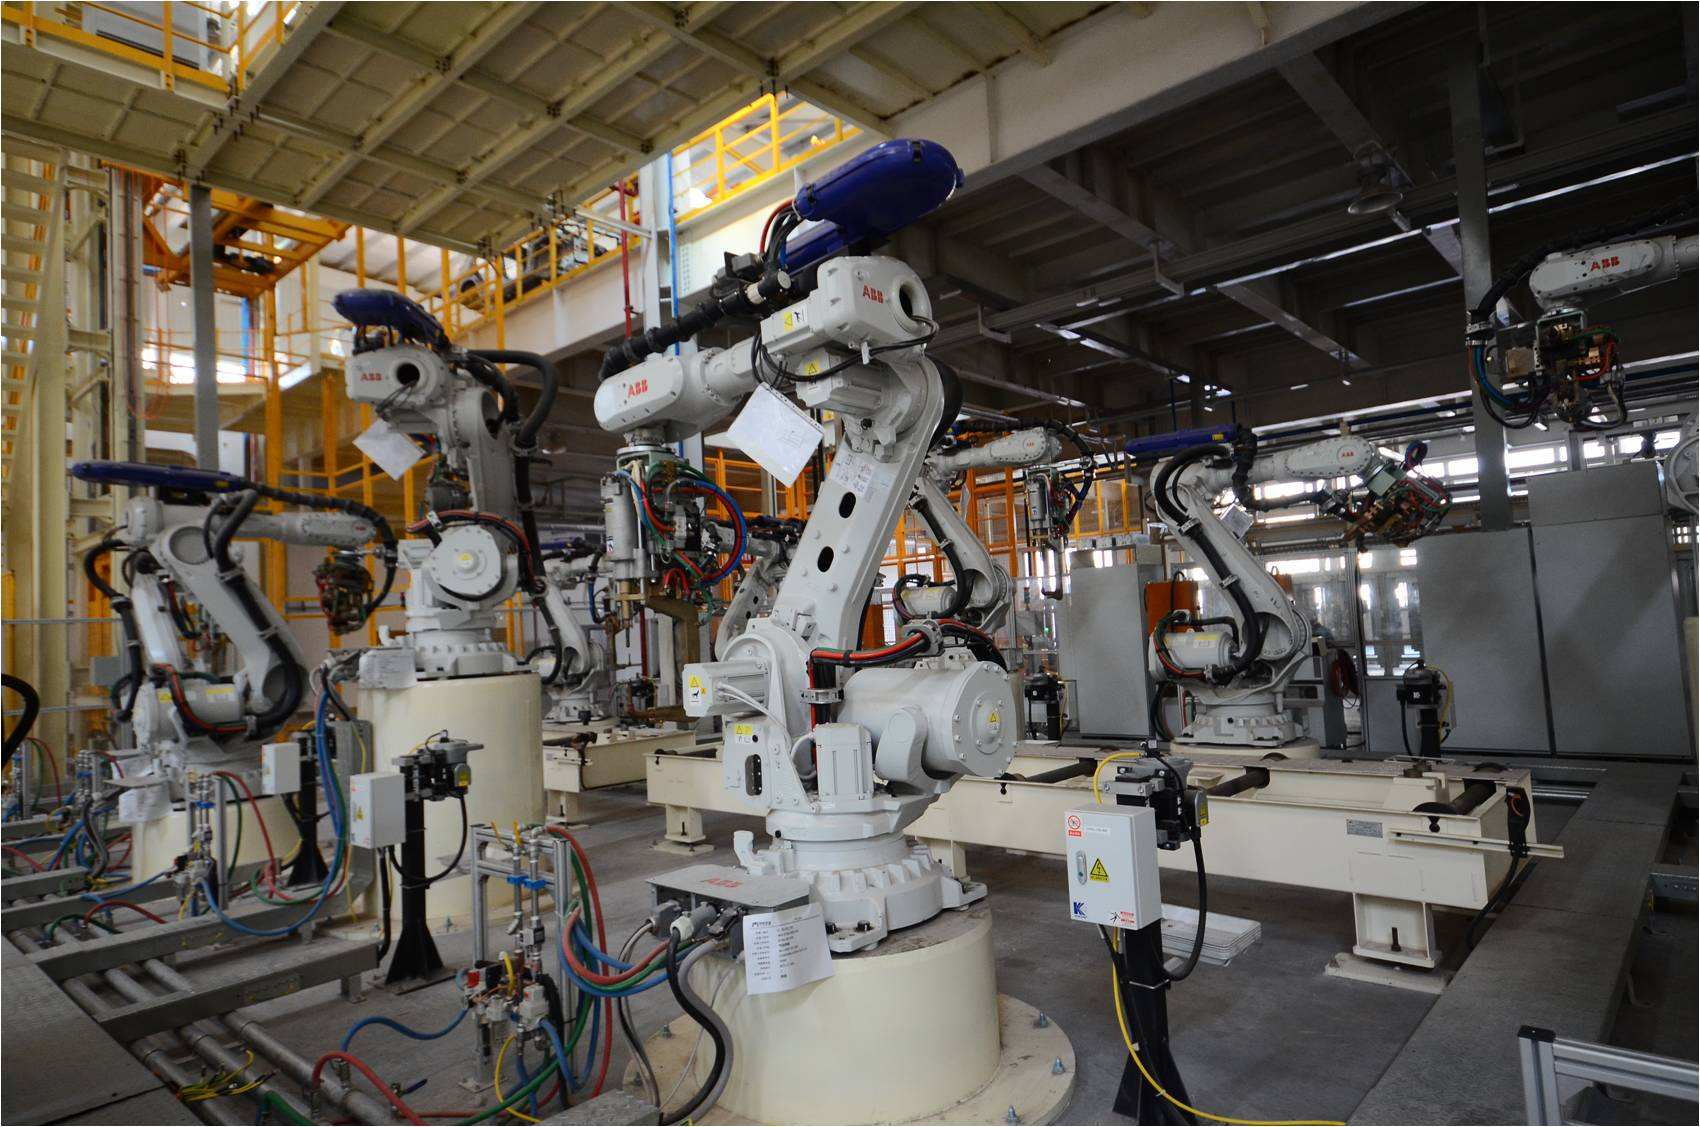
\includegraphics[height=3cm]{abb_car.jpeg}
  \caption{ABB机械臂组成的汽车零件装配产线}
\end{subfigure}
\caption{工业机械臂在流水线上工作}
\label{fig:armcar}
\end{figure}

\begin{figure}
\centering
\begin{subfigure}{.5\textwidth}
  \centering
  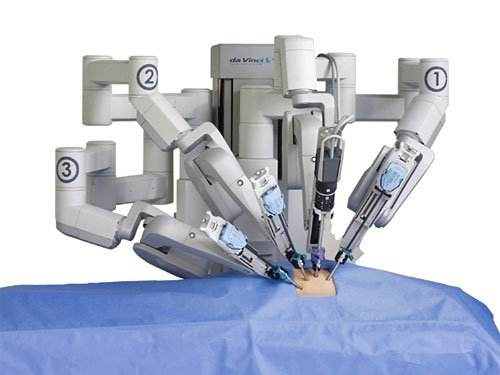
\includegraphics[height=4cm]{davinci.jpeg}
  \caption{达芬奇机器人在工作}
  \label{fig:davinci}
\end{subfigure}%
\begin{subfigure}{.5\textwidth}
  \centering
  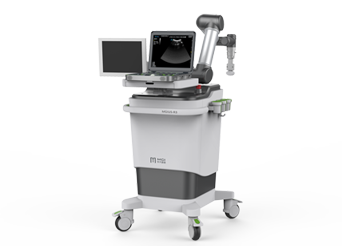
\includegraphics[height=4cm]{huada.png}
  \caption{华大智造的远程超声检测机器人}
  \label{fig:huada}
\end{subfigure}%
\caption{机械臂产品在国内外医疗领域的应用}
\end{figure}



\iffalse % 删掉这些华而不实的玩意儿
    近年来,一些富有展示性的机械臂应用开始逐步面世,例如机器人调酒应用。
    最早引起轰动的是皇家加勒比游轮有限公司在其的最新款邮轮海洋量子号上的“仿生酒吧”中应用了机器人
    调酒师,如图~\ref{fig:liangzi_arm},很快各种调酒机器人被竞相开发出来,如意大利的机器人
    酒吧\ref{fig:italy_arm},拉斯维加斯的机器人调酒师\ref{fig:las_arm},以及我国哈工大开发的
    机器人调酒师\ref{fig:hgd_arm}。尽管机器人调酒目前并不能带来成本或者质量
    上的提升,但是机器人调酒的概念本身富有科技感,新鲜有趣充满噱头,是吸引消费者的一大亮点。


    \begin{figure}
    \centering
    \begin{subfigure}{.5\textwidth}
      \centering
      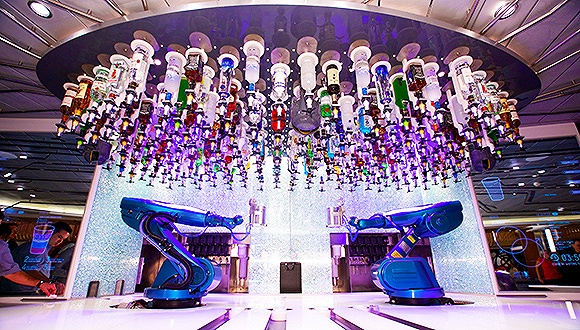
\includegraphics[height=3.5cm]{liangzi_arm.jpg}
      \caption{皇家加勒比海洋量子号的仿生酒吧}
      \label{fig:liangzi_arm}
    \end{subfigure}%
    \begin{subfigure}{.5\textwidth}
      \centering
      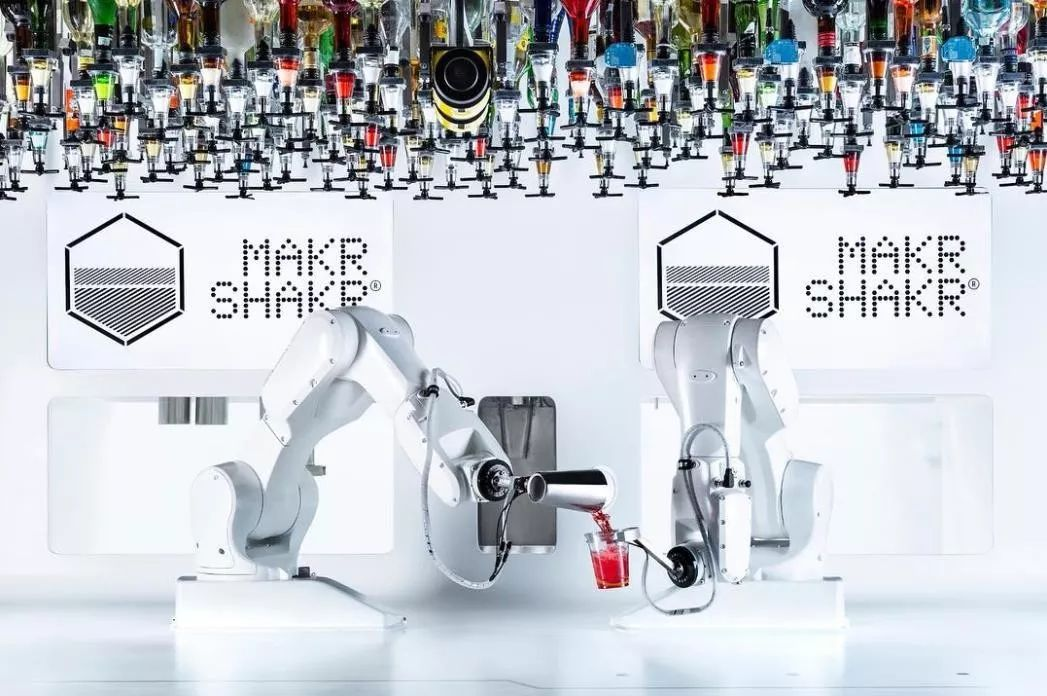
\includegraphics[height=3.5cm]{italy_arm.jpg}
      \caption{意大利The View机器人酒吧}
      \label{fig:italy_arm}
    \end{subfigure}%
    \\
    \begin{subfigure}{.5\textwidth}
      \centering
      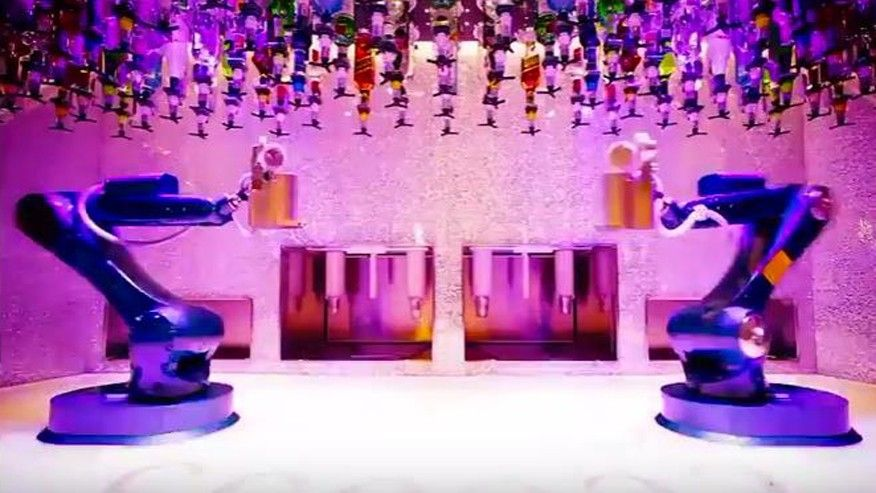
\includegraphics[height=3.5cm]{las_arm.jpg}
      \caption{拉斯维加斯微醺机器人酒吧}
      \label{fig:las_arm}
    \end{subfigure}%
    \begin{subfigure}{.5\textwidth}
      \centering
      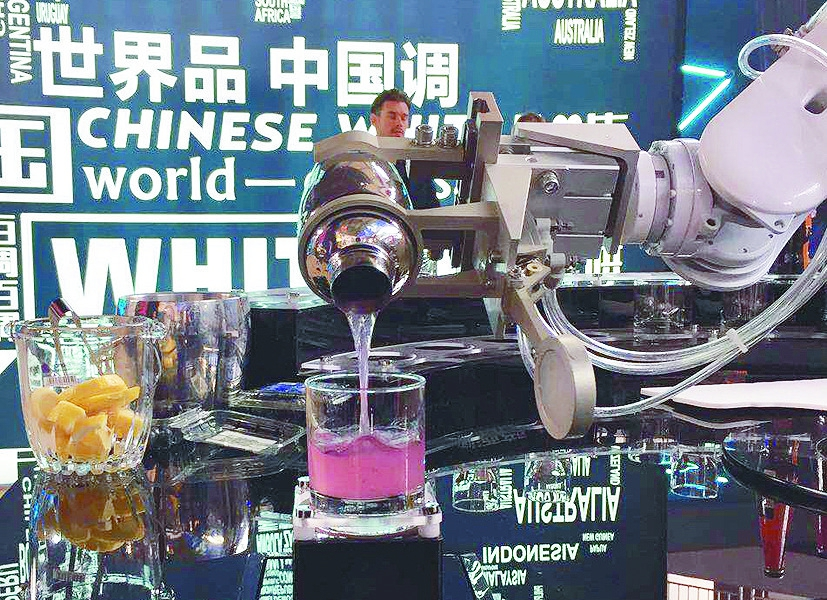
\includegraphics[height=3.5cm]{hgd_arm.jpg}
      \caption{哈工大开发的机器人调酒师}
      \label{fig:hgd_arm}
    \end{subfigure}%
    \caption{机械臂调酒师}
    \end{figure}

\fi

上述这些产品注重控制精度与末端负载,功耗巨大,重量也非常可观,几乎没有移动能力。
尽管工业机器人行业至今已发展多年,体量巨大,技术积累丰厚,但企业的产品研发主要集中在
工业机械臂的硬件性能方面,如提升精度与负载,提升安全性等等。近年来随着电商、物流行业
的迅猛发展,基于机械臂的智能分捡领域开始
蓬勃发展,国内涌现出一批专注物品分捡、分类的创业公司,如深圳蓝胖子机器人~\ref{fig:lanpangzi}、
北京梅卡曼德机器人~\ref{fig:mechmind}等,这些企业专注于算法或者算法硬件集成,致力于
机器人的自动化与智能化。


\begin{figure}
\centering
\begin{subfigure}{.5\textwidth}
  \centering
  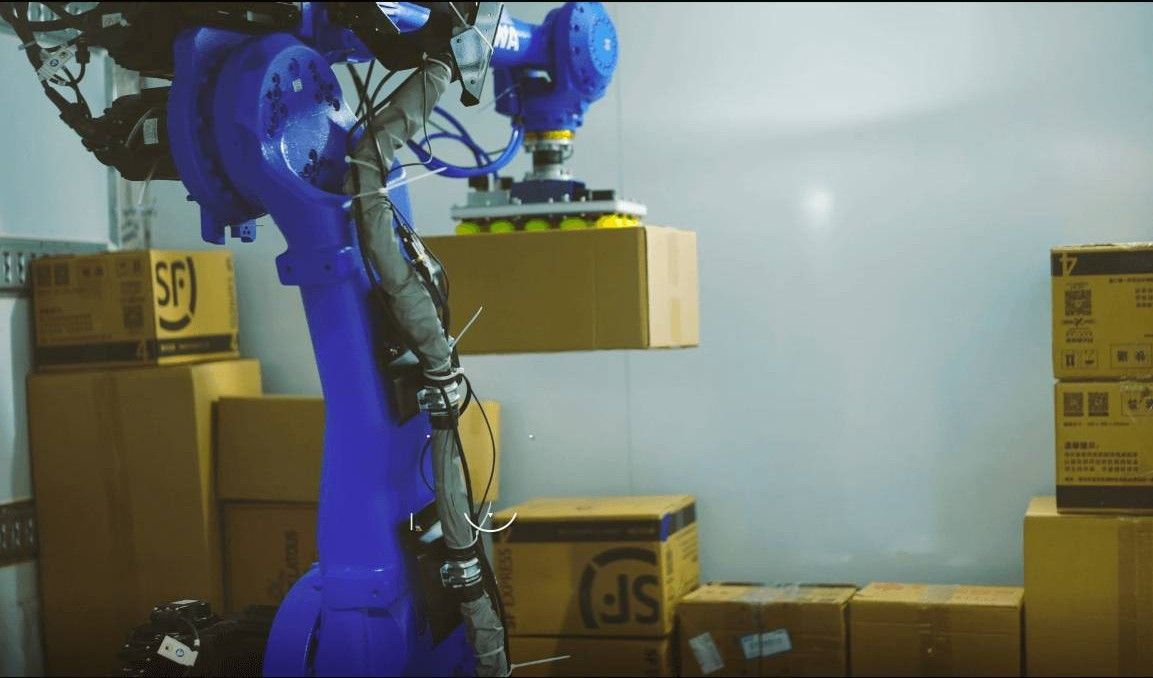
\includegraphics[height=4cm]{lanpangzi_robot.jpeg}
  \caption{蓝胖子机器人研发的机械臂分捡系统}
  \label{fig:lanpangzi}
\end{subfigure}%
\begin{subfigure}{.5\textwidth}
  \centering
  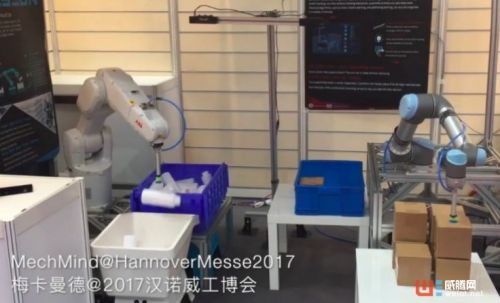
\includegraphics[height=4cm]{mechmind.jpg}
  \caption{梅卡曼德研发的机械臂操作系统在工作}
  \label{fig:mechmind}
\end{subfigure}
\end{figure}

除了专注于操作的工业机械臂,专注移动导航的自动导航车(AGV,Automated Guided Vehicles)
在制造业、运输业也大放异彩。AGV产品最早出现在上世纪50年代,于70年代左右开始应用于
制造业\cite{黄志球2010自动导航车}。按
功能可将AGV分为自动搬运车、自动拖车、自动叉车等几类,或者按照导航方式可分为电磁引导、激光引导、
惯性引导等方式。目前AGV在汽车厂(如通用、丰田、大众等)的制造和装配线上都得到了广泛的使用。
相比于工业机械臂,AGV的机械、电子结构并不复杂,控制算法也相对成熟,制造难度不大。我国的海康威视
就是一个重要的AGV生产商,如图~\ref{fig:haikang}展示了海康威视研发的系列AGV产品。

\begin{figure}
\centering
\begin{subfigure}{.5\textwidth}
  \centering
  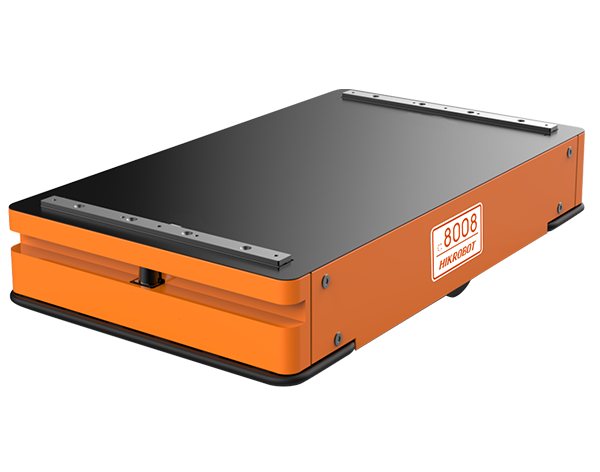
\includegraphics[width=.7\linewidth]{haikang1.png}
  \caption{移载AGV}
\end{subfigure}%
\begin{subfigure}{.5\textwidth}
  \centering
  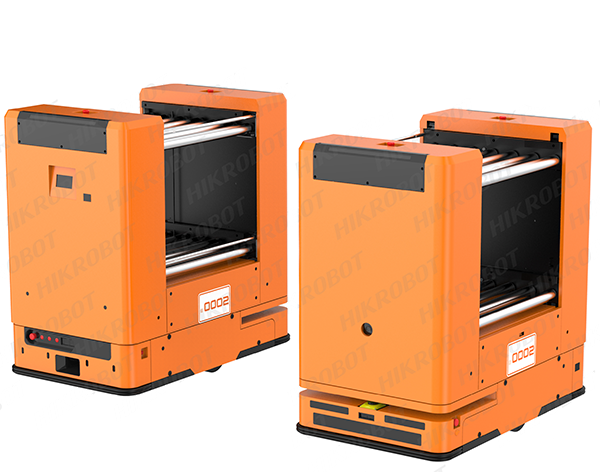
\includegraphics[width=.7\linewidth]{haikang2.png}
  \caption{移载AGV}
\end{subfigure}%
\\
\begin{subfigure}{.5\textwidth}
  \centering
  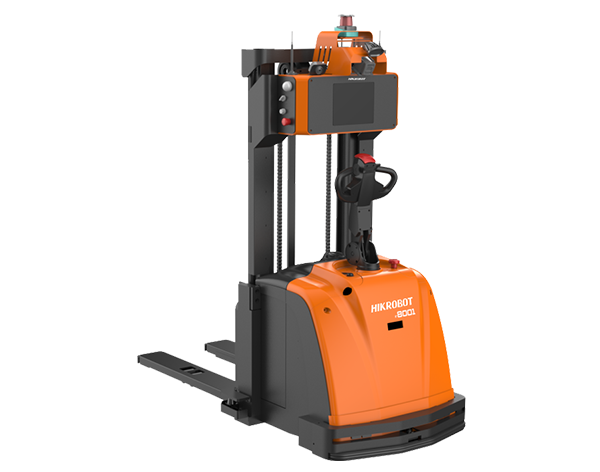
\includegraphics[width=.7\linewidth]{haikang3.png}
  \caption{叉车}
\end{subfigure}%
\begin{subfigure}{.5\textwidth}
  \centering
  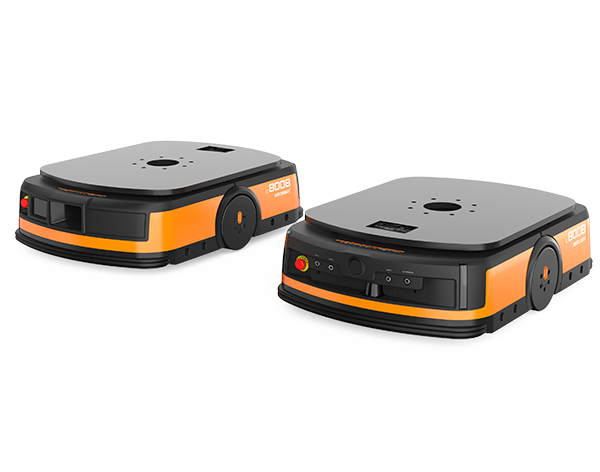
\includegraphics[width=.7\linewidth]{haikang4.png}
  \caption{潜伏系列}
\end{subfigure}%
\caption{海康威视发布的各式AGV产品}
\label{fig:haikang}
\end{figure}

AGV产品除了在制造业广泛应用外,近年来也开始在服务业逐步发展,例如今年来十分火爆的海底捞
机器人餐厅配备了智能AGV送餐员(图~\ref{fig:haidilao}),瑞幸咖啡尝试的无人配送小车
(图~\ref{fig:luckin}),
智行者开发的无人自动清扫车(图~\ref{fig:zhixingzhe}), Yogo Robot开发的写字楼包
裹配送机器人(图~\ref{fig:yogo}),极木科技开发的智能车辆搬动机器人(图~\ref{fig:jimu})
等等。这些产品专注细分领域的需求,有一定的智能处理能力。

\begin{figure}
\centering
\begin{subfigure}{.5\textwidth}
  \centering
  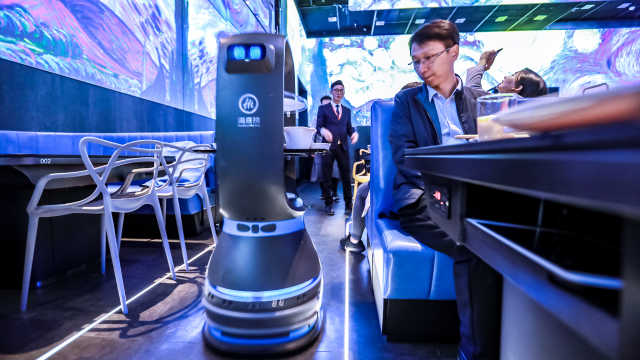
\includegraphics[height=3.5cm]{haidilao.jpg}
  \caption{海底捞送餐机器人}
  \label{fig:haidilao}
\end{subfigure}%
\begin{subfigure}{.5\textwidth}
  \centering
  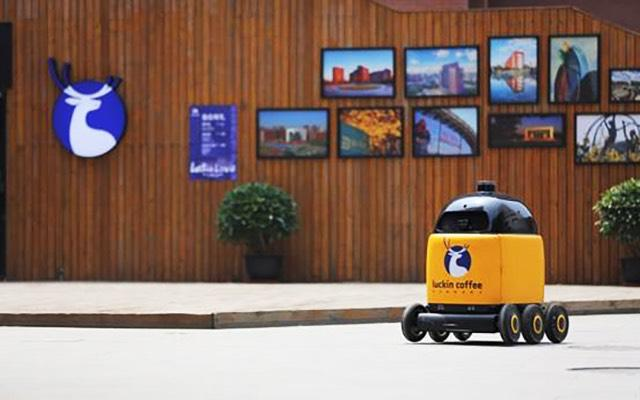
\includegraphics[height=3.5cm]{luckin.jpg}
  \caption{瑞幸咖啡的无人配送车}
  \label{fig:luckin}
\end{subfigure}%
\\
\begin{subfigure}{.5\textwidth}
  \centering
  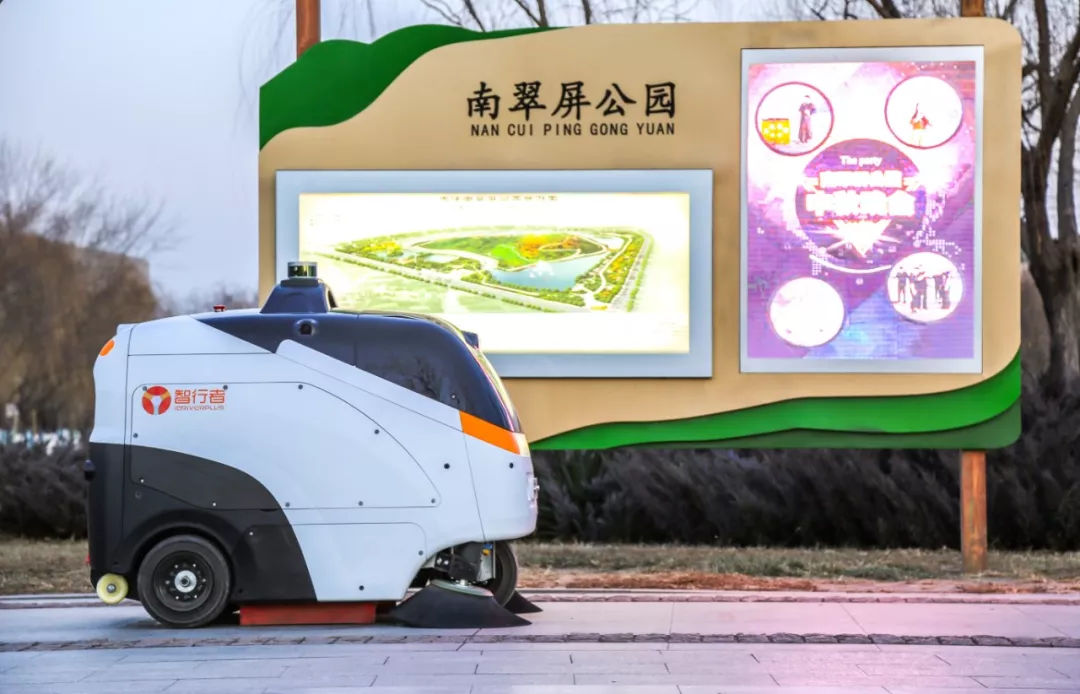
\includegraphics[height=3.5cm]{zhixingzhe.jpg}
  \caption{智行者开发的无人自动清扫车}
  \label{fig:zhixingzhe}
\end{subfigure}%
\begin{subfigure}{.5\textwidth}
  \centering
  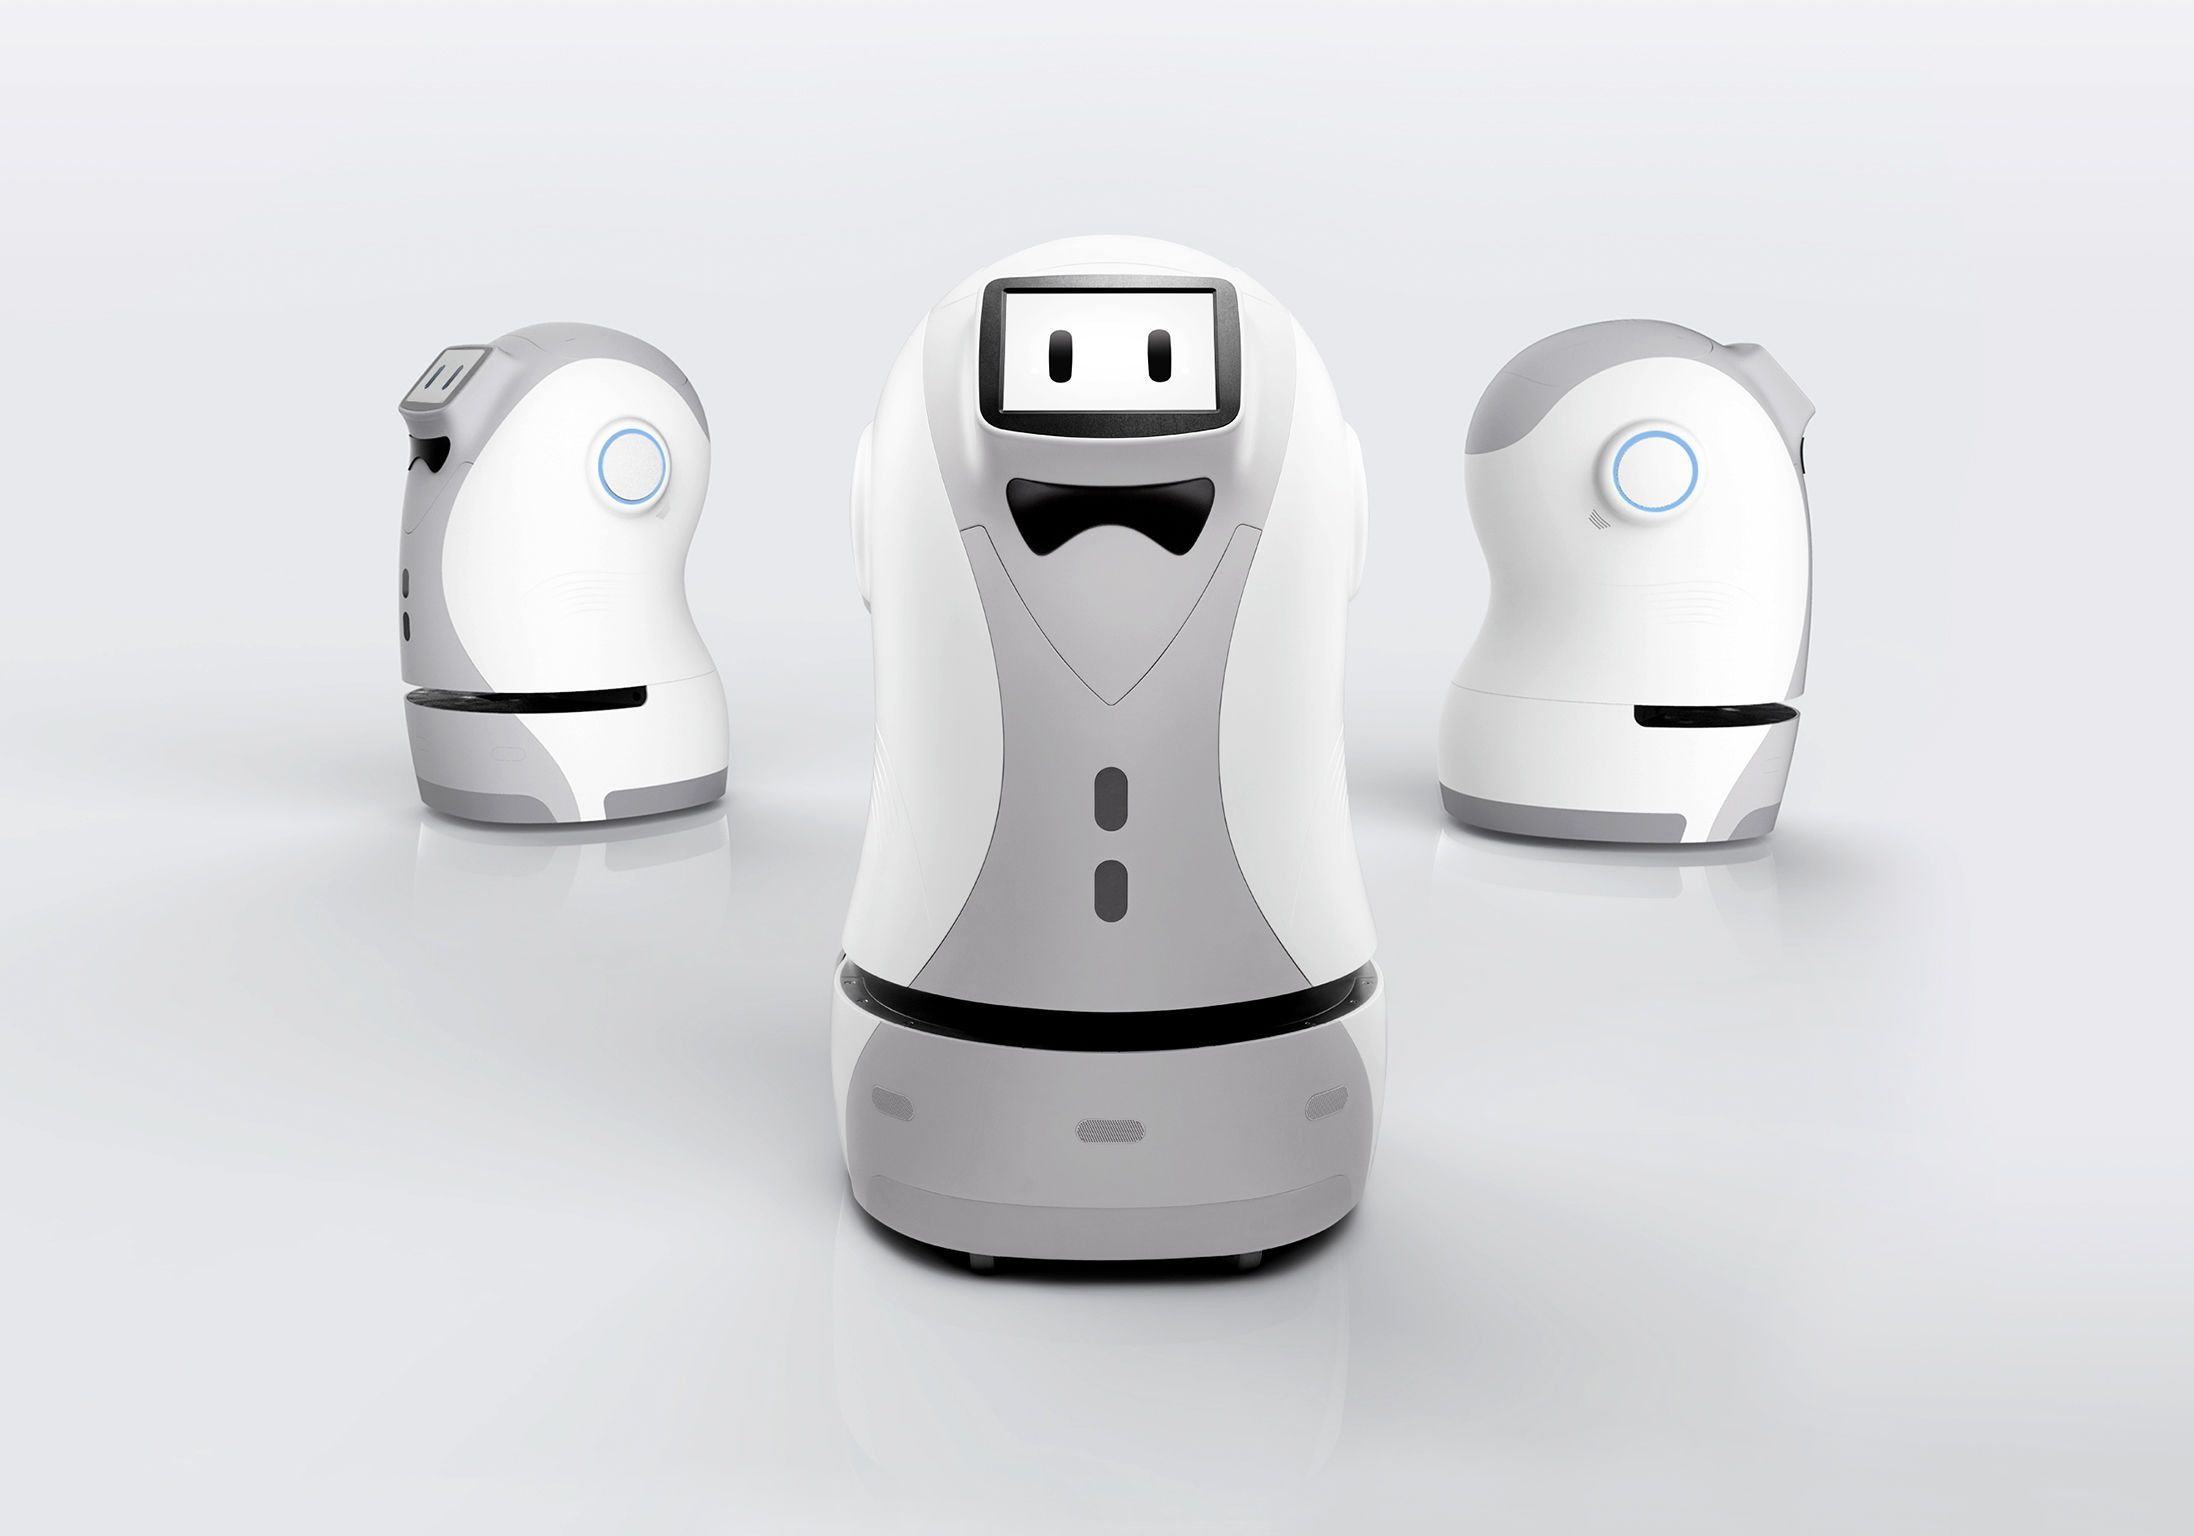
\includegraphics[height=3.5cm]{yogo.jpg}
  \caption{Yogo Robot开发的写字楼包裹配送机器人}
  \label{fig:yogo}
\end{subfigure}%
\\
\begin{subfigure}{.5\textwidth}
  \centering
  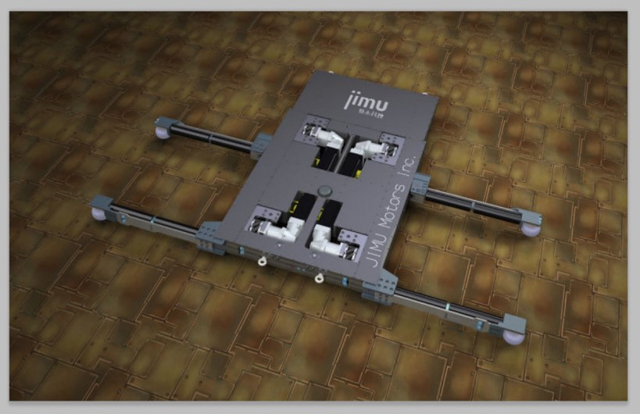
\includegraphics[height=3.5cm]{jimu.jpg}
  \caption{极木科技开发的智能车辆搬动机器人}
  \label{fig:jimu}
\end{subfigure}%
\caption{AGV机器人在服务业的应用}
\end{figure}


移动操作机器人本质上是机械臂产品与AGV的集合,但目前来看其商业应用方向与前两者有极大的区别。
现阶段移动操作机器人领域还没有出现在商业上十分成功的厂商,但是国内外出现了一大批专注这一
领域的创业公司和项目,致力于将移动操作机器人应用到医疗、服务、制造等场景下。例如Diligent Robotics
研发的机器人护士Moxi(如图~\ref{fig:moxi})专注于医院场景下的配送、运输业务;欧
盟发起的旨在推动工业环境中机器人与人写作的”第二双手“(SecondHand)项目的一期项目成
果,AMRAR-6机器人(如图~\ref{fig:armar6})能够在工业环境下与工人协作完成物品的搬动、维修等任务。

\begin{figure}
\centering
\begin{subfigure}{.5\textwidth}
  \centering
  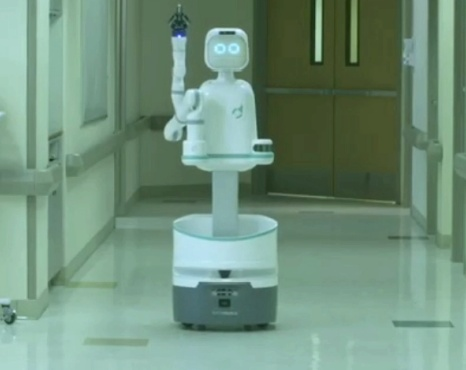
\includegraphics[height=4.2cm]{moxi.jpg}
  \caption{Moxi机器人护士}
  \label{fig:moxi}
\end{subfigure}%
\begin{subfigure}{.5\textwidth}
  \centering
  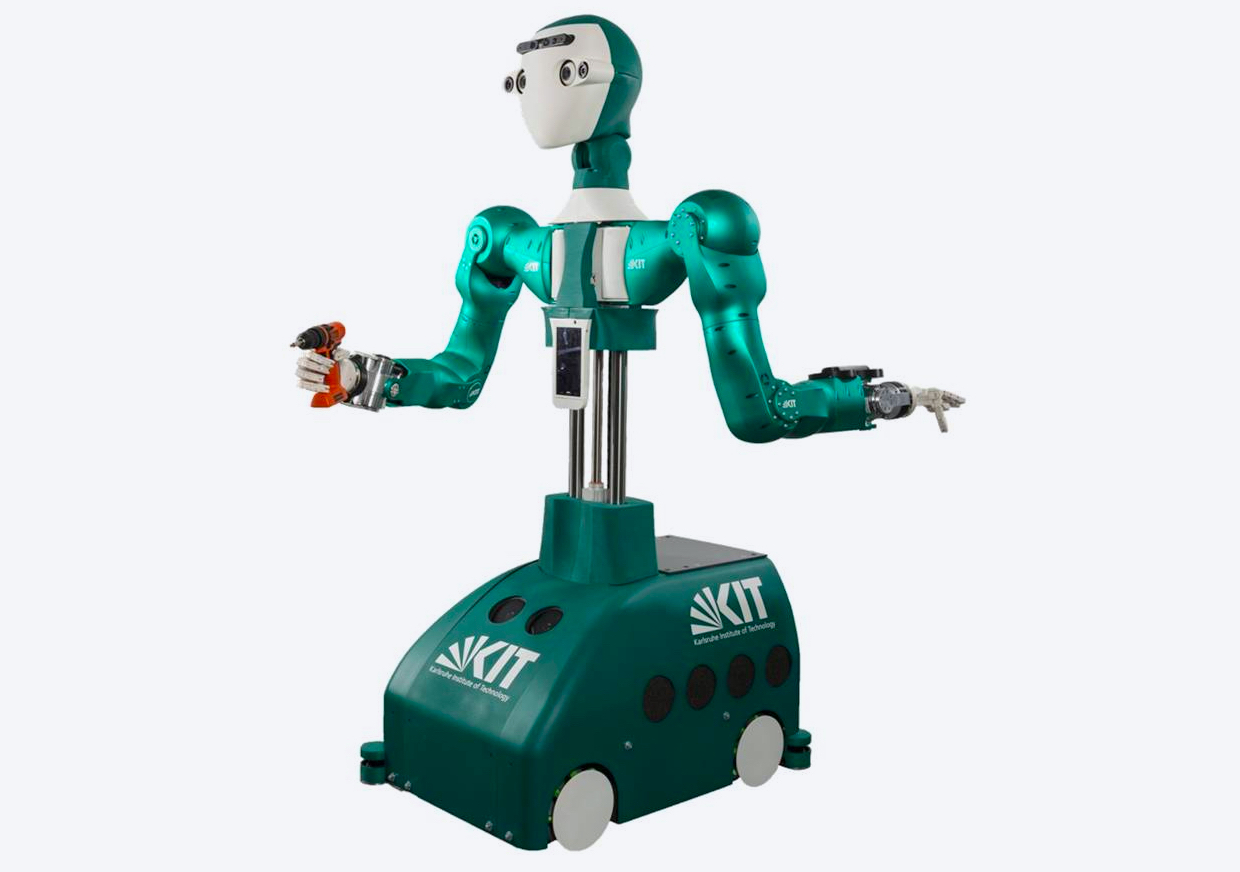
\includegraphics[height=4.2cm]{armar6.jpeg}
  \caption{ARMAR-6仿人机器人}
  \label{fig:armar6}
\end{subfigure}%
\caption{国内外创业公司研发的医疗移动操作机器人}
\end{figure}

除上述两例面向特定任务的移动机器人外,产业界还有一部分产品定位为“仿人”的具有社交属性的服务
机器人,例如日本Toyota公司面对人口老龄化现象推出的家庭照料机器人HSR(Human Support Robot)\ref{fig:hsr},
以及Softbank Robotic发布的Pepper机器人\ref{fig:pepper}。这些机器人大都行动笨拙,但是有双臂、
手、头等和人类身体结构对应的机械结构,并且有一定的交互能力。

\begin{figure}
\centering
\begin{subfigure}{.5\textwidth}
  \centering
  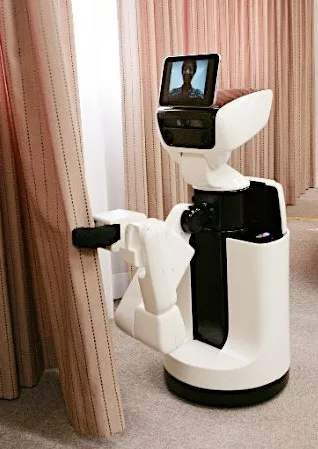
\includegraphics[height=5cm]{hsr.jpeg}
  \caption{Toyota Human Support Robot}
  \label{fig:hsr}
\end{subfigure}%
\begin{subfigure}{.5\textwidth}
  \centering
  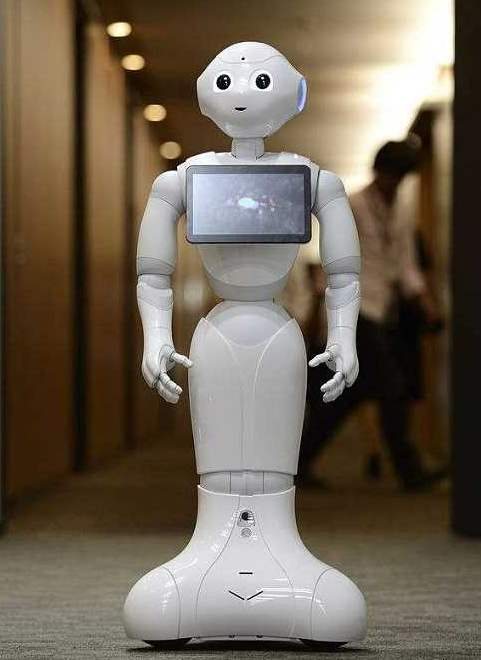
\includegraphics[height=5cm]{pepper.jpeg}
  \caption{Softbank Robotics Pepper}
  \label{fig:pepper}
\end{subfigure}
\label{fig:hsr_pepper}
\caption{仿人机器人产品}
\end{figure}

除了上述商业应用比较明确的公司以及产品外,国际上大名顶顶的波士顿动力公司(Boston Dynamics)也
研究发布了几款轮式移动操作机器人(如图~\ref{fig:bd_wheel}),和以大狗为移动平台挂载轻量
级机械臂的机器人(如图~\ref{fig:bd_dog})。这些机器人在运动控制上均达到了极高的水平,为
移动操作机器人的运动性能评价设定了新的标杆。

\begin{figure}
\centering
\begin{subfigure}{.5\textwidth}
  \centering
  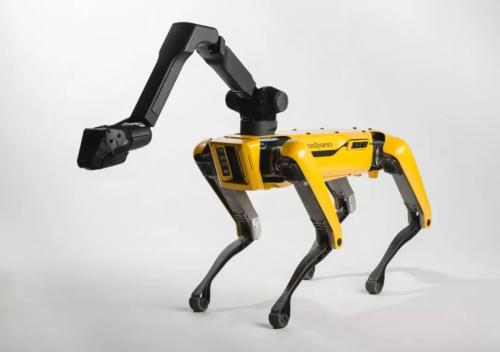
\includegraphics[width=.6\linewidth]{bd_dog.jpg}
  \caption{SPOTMINI + Arm大狗机器人}
  \label{fig:bd_dog}
\end{subfigure}%
\begin{subfigure}{.5\textwidth}
  \centering
  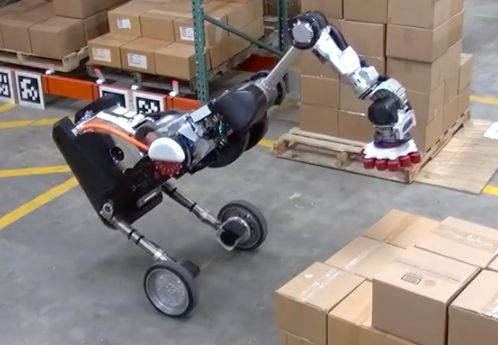
\includegraphics[width=.6\linewidth]{bd_wheel.jpg}
  \caption{仓储搬运机器人Handle}
  \label{fig:bd_wheel}
\end{subfigure}
\caption{波士顿动力发布的移动操作机器人产品}
\end{figure}


\section{移动操作机器人国内外研究现状}
\label{cha:research}

机器人领域中学术界的研究总是走在工业界前面,移动操作机器人方向也不例外。最早的工业
机械臂于1969年由Victor Scheinman发明,称为“斯坦福机械臂”,随后Victor Scheinman在
MIT AI Lab设计了被成为“MIT arm”的机械臂并在一些公司的支持下开发了Puma机器人\cite{huangxihuanReview},
机器人最初诞生自高校的实验室里。在50年后的今天,学术界的研究依然指引着机器人发展的
方向。随着计算机技术的不断发展,深度学习以及各类控制算法的成熟,研究者们开始将目光
聚焦于提升机器人的“智能性”以及它的泛化性上。

学术领域在探索各式感知、控制、交互方法的同时,也自研或者培育了许多移动操作机器人产品。
这些产品机器人不但对领域内前沿的设计思想进行实践、对前沿的传感器进行尝试,方便了广大
研究人员,有些甚至取得了商业上的成功。例如在开源机器人领域著名的PR2机器人
(如图~\ref{fig:pr2})以及TurtleBot(如图~\ref{fig:turtlebot})机器人平台。

\begin{figure}
\centering
\begin{subfigure}{.6\textwidth}
  \centering
  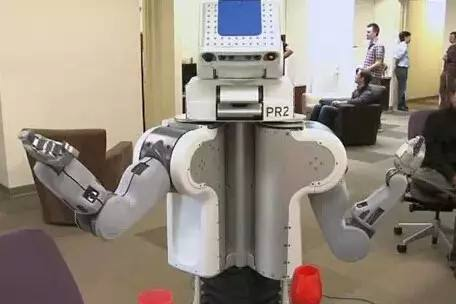
\includegraphics[height=4cm]{pr2.jpeg}
  \caption{PR2服务机器人}
  \label{fig:pr2}
\end{subfigure}%
\begin{subfigure}{.4\textwidth}
  \centering
  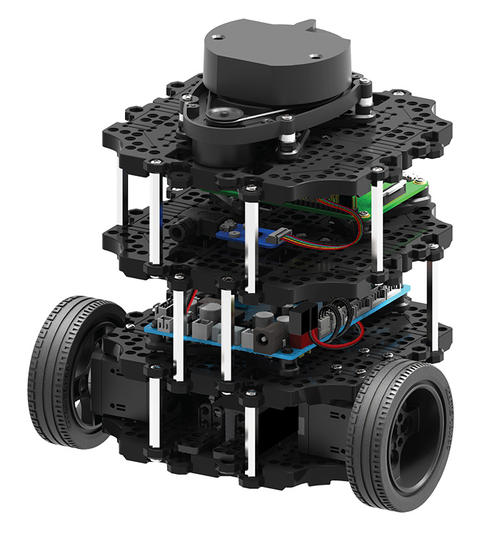
\includegraphics[height=4cm]{turtlebot3.jpg}
  \caption{turtlebot3机器人}
  \label{fig:turtlebot}
\end{subfigure}
\caption{学术机器人平台}
\end{figure}

为了统一机器人算法研究的编程平台,降低方法的复现难度,促进社区的健康发展。广大机器人
研究学者们也参与推动维护了多个开源的机器人编程框架,其中包括应用广泛的ROS
(Robot Operating System)\cite{quigley2009ros},YARP
(Yet another robot platform)\cite{metta2006yarp}等框架。这些开源框架为社区提供了
极大的发展便利,同时某些面向学术研究的移动机器人操作平台也通过捆绑支持这些机器人
编程框架取得了商业上的成功,例如前文提到的PR2和TurtleBot机器人;Universal Robotics
研发的URx系列机械臂(图~\ref{fig:urx}); 以及国内的autolabor四轮
差速车(图~\ref{fig:autolaborpro1} ~\ref{fig:autolabor})等等产品。


\begin{figure}
\centering
\begin{subfigure}{.6\textwidth}
  \centering
  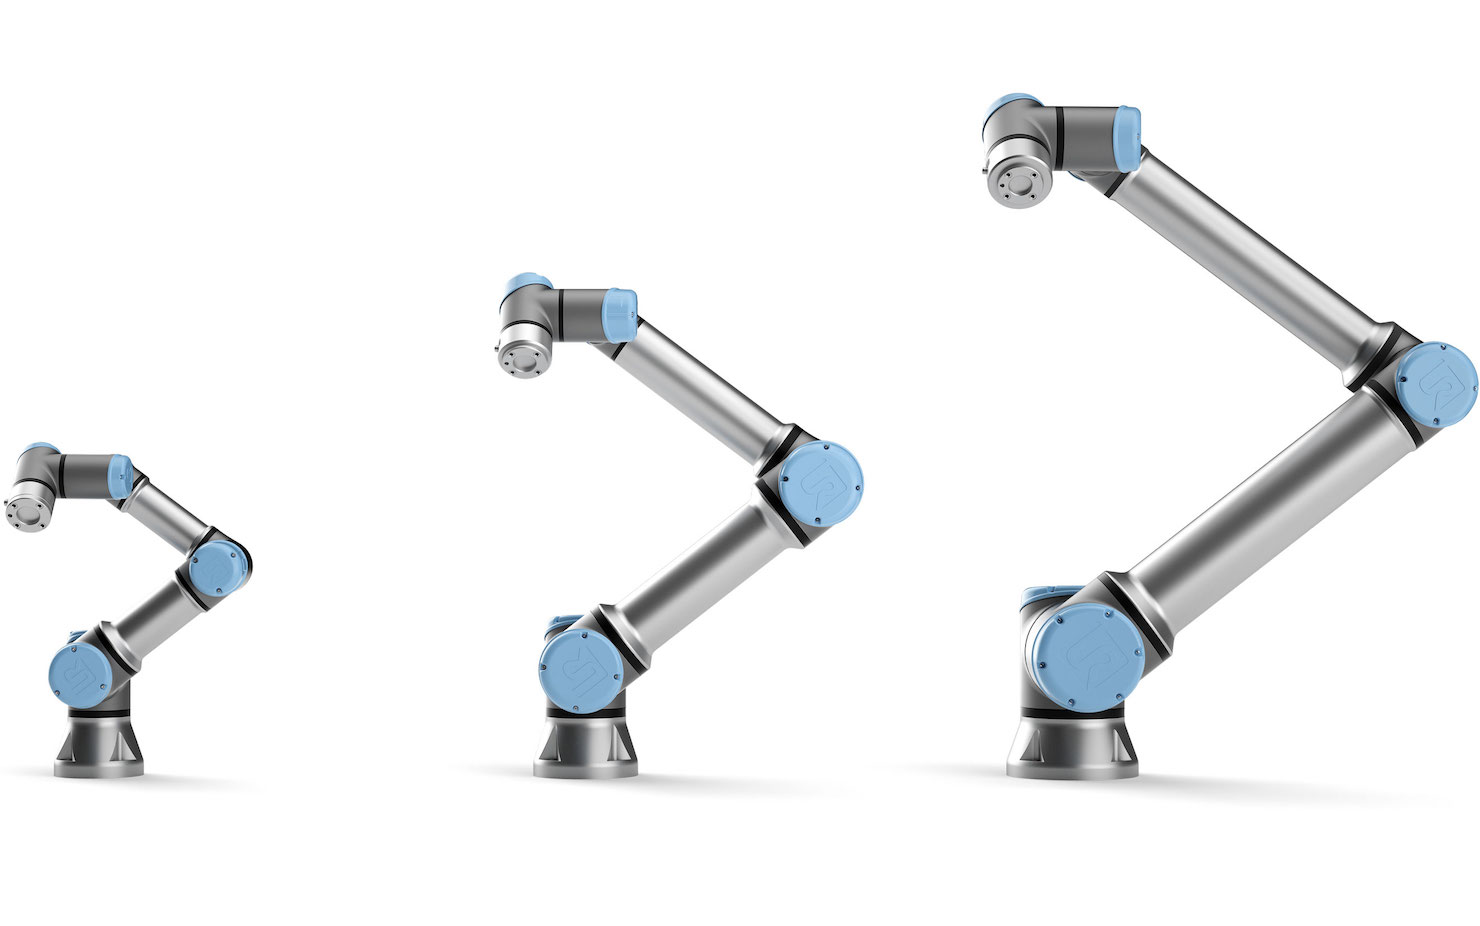
\includegraphics[height=3.5cm]{ur_series.jpg}
  \caption{Universal Robotics研发的系列UR机械臂}
  \label{fig:urx}
\end{subfigure}%
\begin{subfigure}{.4\textwidth}
  \centering
  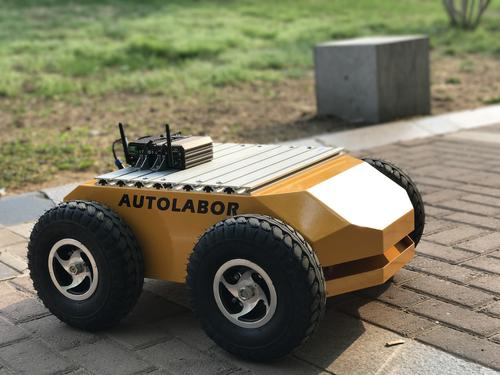
\includegraphics[height=3.5cm]{autolaborpro1.jpg}
  \caption{Autolabor 大负载四轮差速车}
  \label{fig:autolaborpro1}
\end{subfigure}
\begin{subfigure}{.5\textwidth}
  \centering
  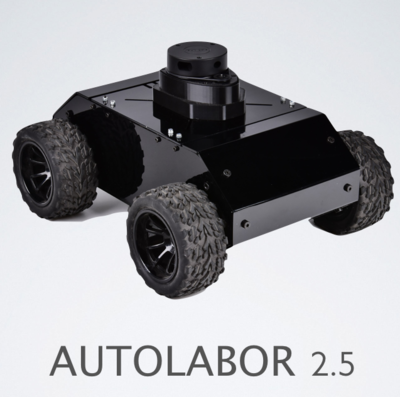
\includegraphics[width=.6\linewidth]{autolabor.jpg}
  \caption{Autolabor小型四轮差速平台}
  \label{fig:autolabor}
\end{subfigure}
\caption{支持ROS平台的机器人产品}
\end{figure}


机器人算法一直是科研领域的研究热点,按照功能可以将机器人相关的算法分为感知和控制两部分。
感知方向包括物品的检测、分类、定位等功能,得益于深度神经网络的快速发展,机器人的感知能力
近年来有了飞速的提高,借助经典的视觉检测方法配合机械臂规划方法实现的快速自动分捡方案
在各大比赛中不断出现。借助深度学习(如图~\ref{fig:img_seg})或者传统视觉方法、点云
处理方法(如图~\ref{fig:pc_seg})实现的拾取平面检测,抓取
点寻找,夹爪位姿寻找算法也不断涌现,并且取得了非常好的效果。

\begin{figure}
\centering
\begin{subfigure}{.5\textwidth}
  \centering
  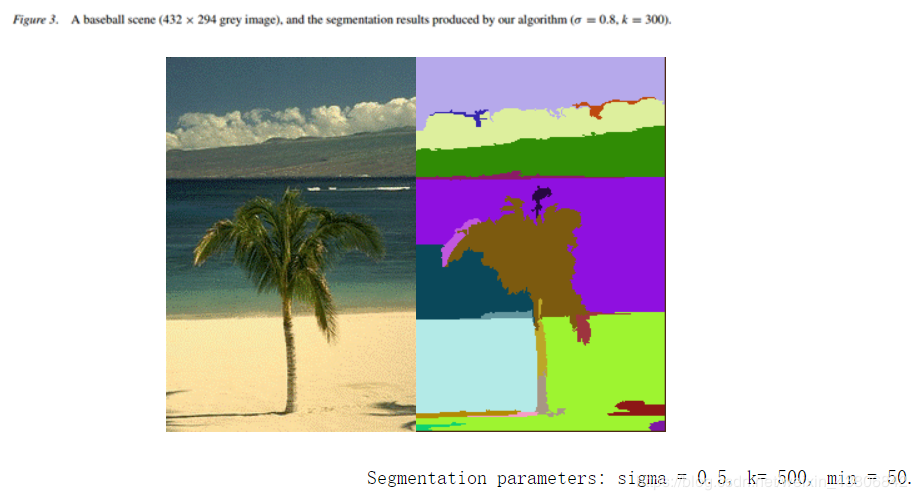
\includegraphics[height=4cm]{img_seg.jpg}
  \caption{基于图片的物品分割识别}
  \label{fig:img_seg}
\end{subfigure}%
\begin{subfigure}{.5\textwidth}
  \centering
  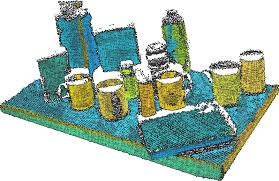
\includegraphics[height=4cm]{pc_seg.jpeg}
  \caption{基于点云的物品分割效果}
  \label{fig:pc_seg}
\end{subfigure}
\caption{学术机器人平台}
\end{figure}


在导航定位方面,SLAM技术( simultaneous localization and mapping,即时定位与地图构建)
日趋成熟,基于视觉、点云或者多传感器融合的算法不断出现,视觉方面,直接法、特征点法
或者半直接的算法大量增加,特别的基于优化的方案有了长足的发展,被认为在未来的SLAM领域能够取代
滤波算法,如基于特征点法的ORB-SLAM\cite{mur2015orb},视觉与IMU融合的VINS\cite{qin2018vins},
半直接法的SVO\cite{forster2014svo},稀疏直接法的DSO\cite{engel2017direct} 等等,
如图~\ref{fig:slams};基于雷达的各类
SLAM算法进展也十分迅速,如基于粒子滤波的Gmapping\cite{grisettiyz2005improving},基于优化
的loam\cite{zhang2014loam},基于优化以及子图的Cartographer\cite{hess2016real}等等。激光
SLAM主要以产出2D地图和位姿为主,其算法结果可视化效果大多很相似,如图~\ref{fig:lidar_slams}

\begin{figure}
\centering
\begin{subfigure}{.6\textwidth}
  \centering
  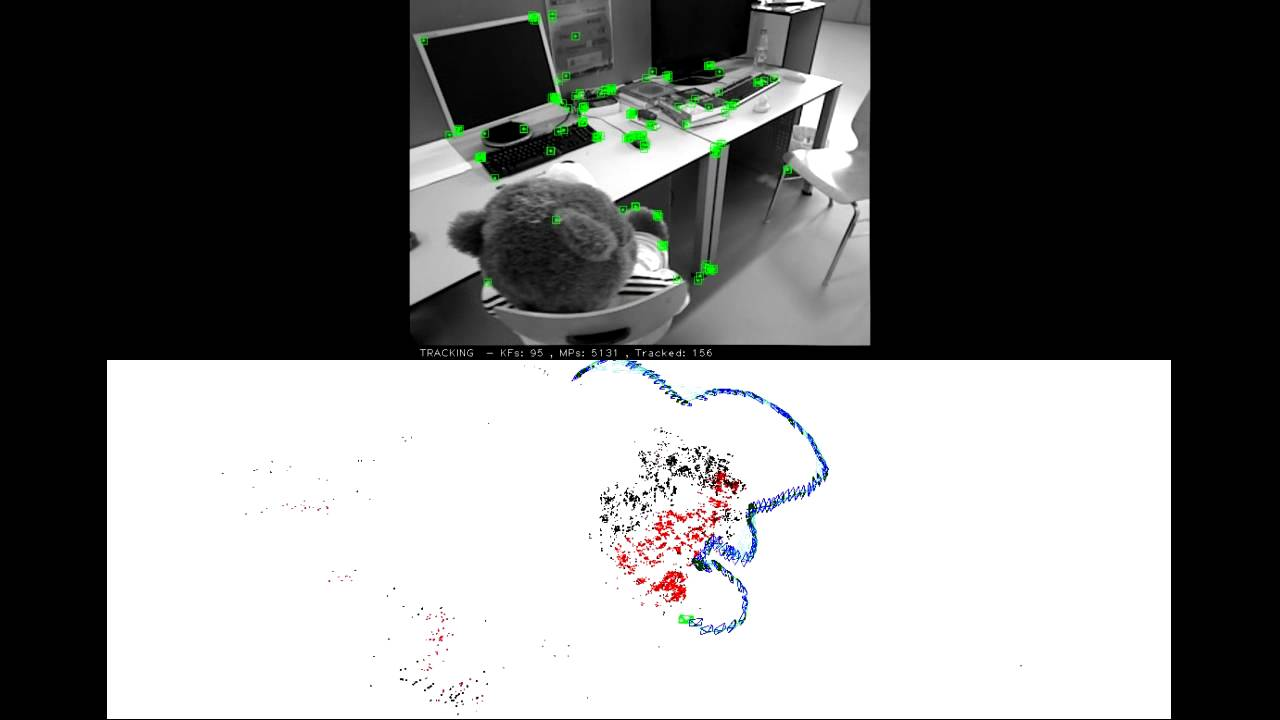
\includegraphics[height=3.5cm]{orb.jpg}
  \caption{ORB-SLAM}
\end{subfigure}%
\begin{subfigure}{.4\textwidth}
  \centering
  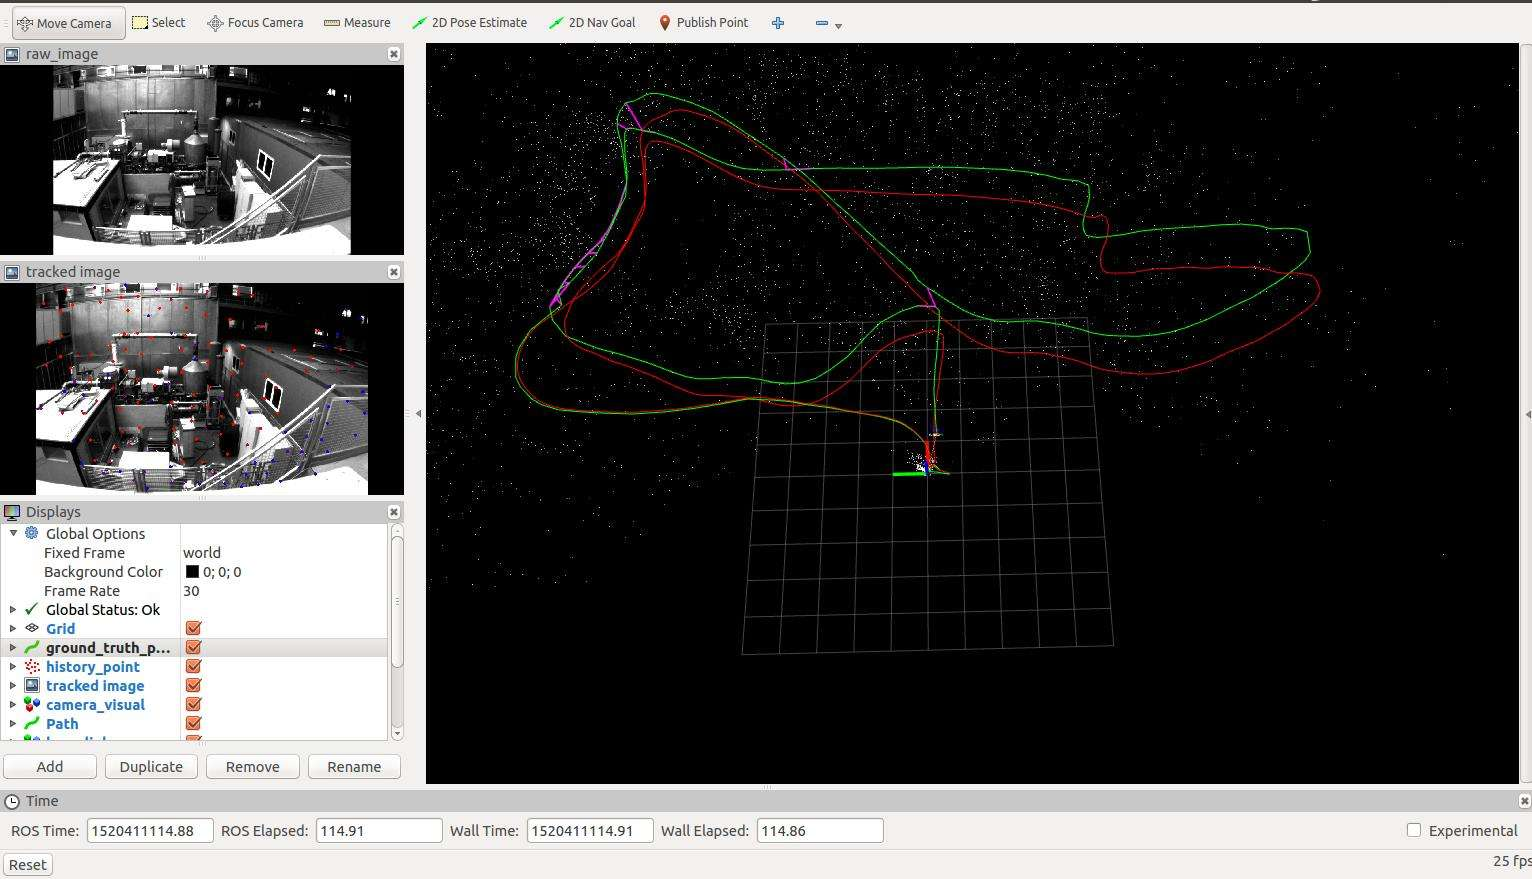
\includegraphics[height=3.5cm]{vins.jpeg}
  \caption{VINS-Mono}
\end{subfigure}
\\
\begin{subfigure}{.59\textwidth}
  \centering
  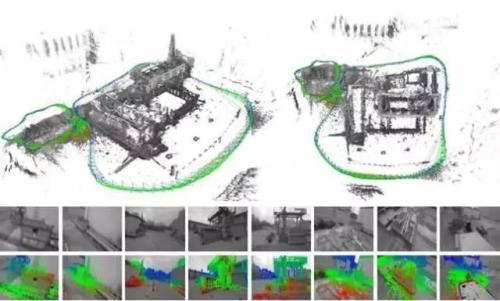
\includegraphics[height=3.2cm]{svo.jpg}
  \caption{SVO}
\end{subfigure}
\begin{subfigure}{.4\textwidth}
  \centering
  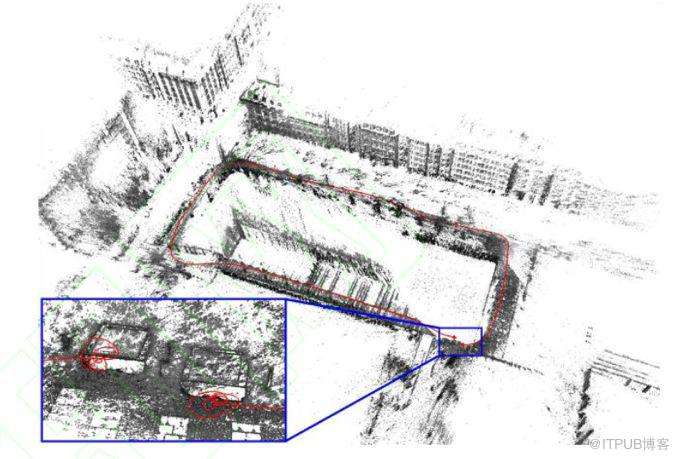
\includegraphics[height=3.2cm]{dso.jpeg}
  \caption{DSO}
\end{subfigure}
\caption{基于视觉的各种SLAM算法效果图}
\label{fig:slams}
\end{figure}


\begin{figure}
\centering
\begin{subfigure}{.5\textwidth}
  \centering
  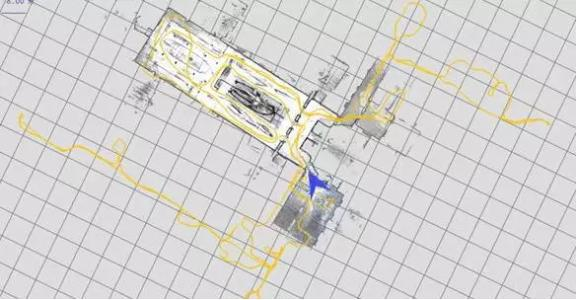
\includegraphics[height=3.7cm]{cartographer.jpg}
  \caption{雷达生成2D地图的可视化效果}
\end{subfigure}%
\begin{subfigure}{.5\textwidth}
  \centering
  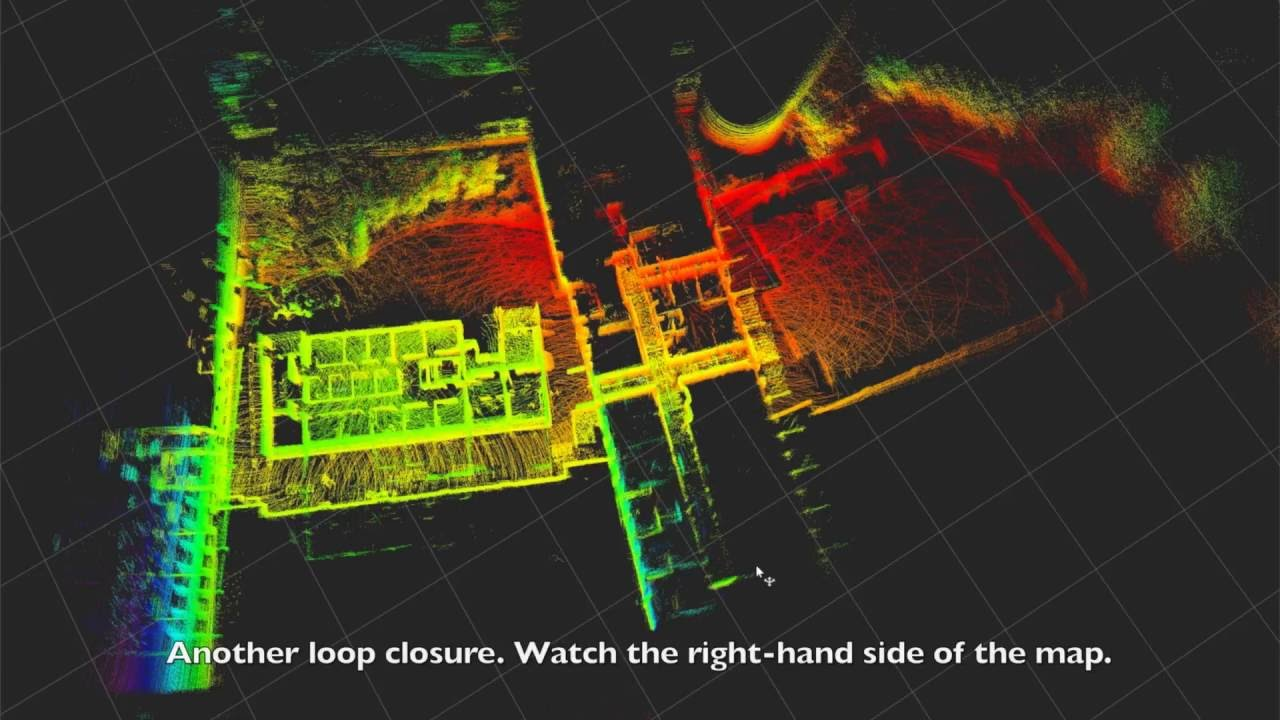
\includegraphics[height=3.7cm]{cartographer3d.jpg}
  \caption{多线激光雷达生成的3D效果图}
\end{subfigure}
\caption{基于雷达的SLAM算法效果图}
\label{fig:lidar_slams}
\end{figure}


格式SLAM算法不断提高机器人主动定位的精度与鲁帮性的同时,导航算法的进步主要体现
在控制框架的创新和完善上,经过数十年的努力,机器人社区在导航方面已经形成了较为稳定的一套
方法,即基于Costmap的分层地图维护方法\cite{lu2014layered}和分别负责路径生成与控制命令
生成的双规划器算法\cite{guimaraes2016ros}。目前
在静态环境中的灵活避障导航问题已经基本被解决\cite{Zhou2017A}。 此外增强学习在机器人控制
上的应用也成为近年来算法方向的研究热点\cite{schaal2002learning}。

机械臂控制算法是机器人算法领域的一大方向,由于现代机械臂自由度高,冗余程度大,状态空间大,
对机械臂的规划算法提出了严峻挑战。学术界不断提出新的机械臂规划算法例如基于梯度优化的机械臂
路径寻找算法 CHOMP\cite{ratliff2009chomp},随机路径优化算法 STOMP\cite{kalakrishnan2011stomp}
等等。同时,一些维护机械臂相关算法 的开源库也迅速兴起,比如维护随机采样规划器的OMPL
(The Open Motion Planning Library)\cite{sucan2010open},
基于搜索算法的SBPL(The Search Based Planning Library)\cite{likhachev2014sbpl},以及
用于碰撞检测的FCL(The Fast Collision Library)\cite{pan2012fcl}。随着这些支撑组件的不断
成熟,一些集运动学解算、路径生成、碰撞检测功能于一体的一站式的机械臂规划框架也开始出现,
如基于ROS的MoveIt!\cite{chitta2012moveit}, V-REP等等,如图~\ref{fig:moveit_vrep}

\begin{figure}
\centering
\begin{subfigure}{.5\textwidth}
  \centering
  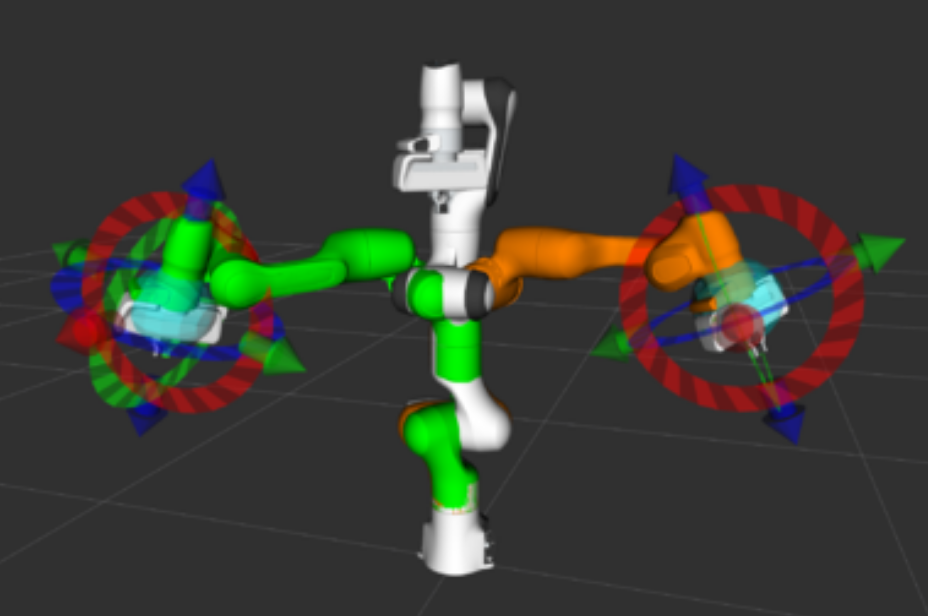
\includegraphics[height=4cm]{moveit.png}
  \caption{MoveIt!工作时的可视化窗口}
\end{subfigure}%
\begin{subfigure}{.5\textwidth}
  \centering
  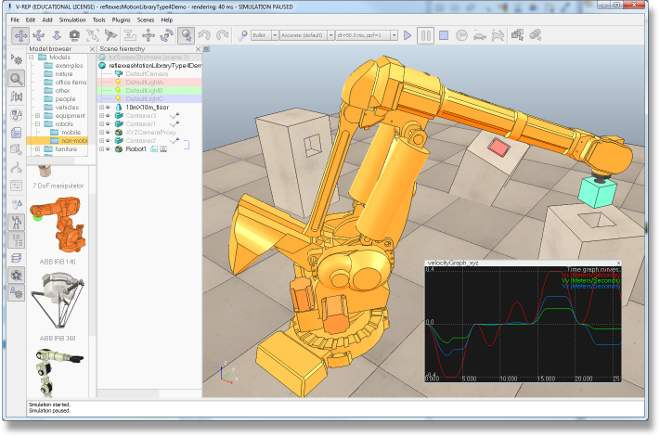
\includegraphics[height=4cm]{vrep.jpeg}
  \caption{V-REP可视化窗口}
\end{subfigure}
\caption{开源的机械臂规划框架}
\label{fig:moveit_vrep}
\end{figure}


为促进研究成果在实际场景中的应用,各大公司会议等组织举办了许多世界级的面向特定场景的
机器人大赛,其中著名的有Amazon Picking Challenge\cite{wurman2016amazon},
RoboCup@Home\cite{wisspeintner2009robocup},IROS Manipulation Competition\cite{moon2017iros}。
这些比赛极大的促进了机器人社区的交流,在比赛期间也涌现出了许多优秀的机器人设计以及
方法。下面以RoboCup@Home为例详细的介绍机器人赛事如何组织及促进学术的发展交流。

RoboCup@Home比赛已经培育起一个完善的社区,每年RoboCup@Home的比赛任务
即由社区相关人员协助商议决定,RoboCup@Home组委会共同维护一份RuleBook\cite{rulebook}
,组委会成员
使用GitHub完成RuleBook的编写任务,该仓库是完全开放且欢迎参赛者提交修改与贡献的。
RoboCup@Home组委会中,设有专门的任务制定部门Technical Committee(TC),这部分成员
大都有深厚的相关从业背景和多年的研究经验,另外有一部分成员来自各个主力参赛队伍的
核心开发人员(比如本文作者作为Tinker机器人的主要程序员参与了2020年的TC工作),以
确保比赛规则同时兼顾学科研究热点和可完成性。

随着机器人行业相关技术的不断发展,RuleBook中的任务也在每年更新,并且向着越来越复杂、
越来越贴近真实生活场景的方向演进。在多年的比赛中,组委会在任务内容、任务形式上也作出
了很多改进与尝试,2019年的RoboCup@Home比赛就及其大胆的将任务数量进行了爆炸式的扩容,
尝试了很多新的复杂的任务,其中有一些被证明并不成功,因此2020年的规则制作过程中又将
不合理的任务去除,将任务数量固定为Stage I 5个,Stage II 4个。 在RoboCup@Home赛场上
出现了大量设计新奇,功能多样的机器人(如图~\ref{fig:other_teams})。

\begin{figure}
    \centering
    \begin{minipage}{.45\linewidth}
            \begin{subfigure}[t]{.9\linewidth}
                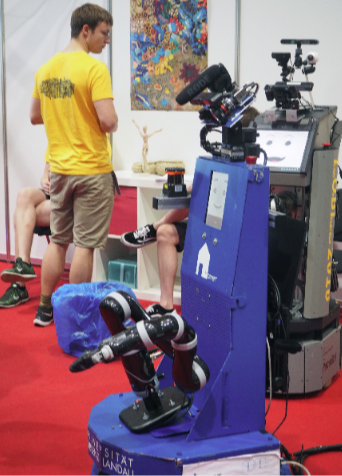
\includegraphics[width=\textwidth]{homer.png}
                \caption{homer@ UniKoblenz}
            \end{subfigure}
    \end{minipage}
    \begin{minipage}{.45\linewidth}
        \begin{subfigure}[t]{.8\linewidth}
            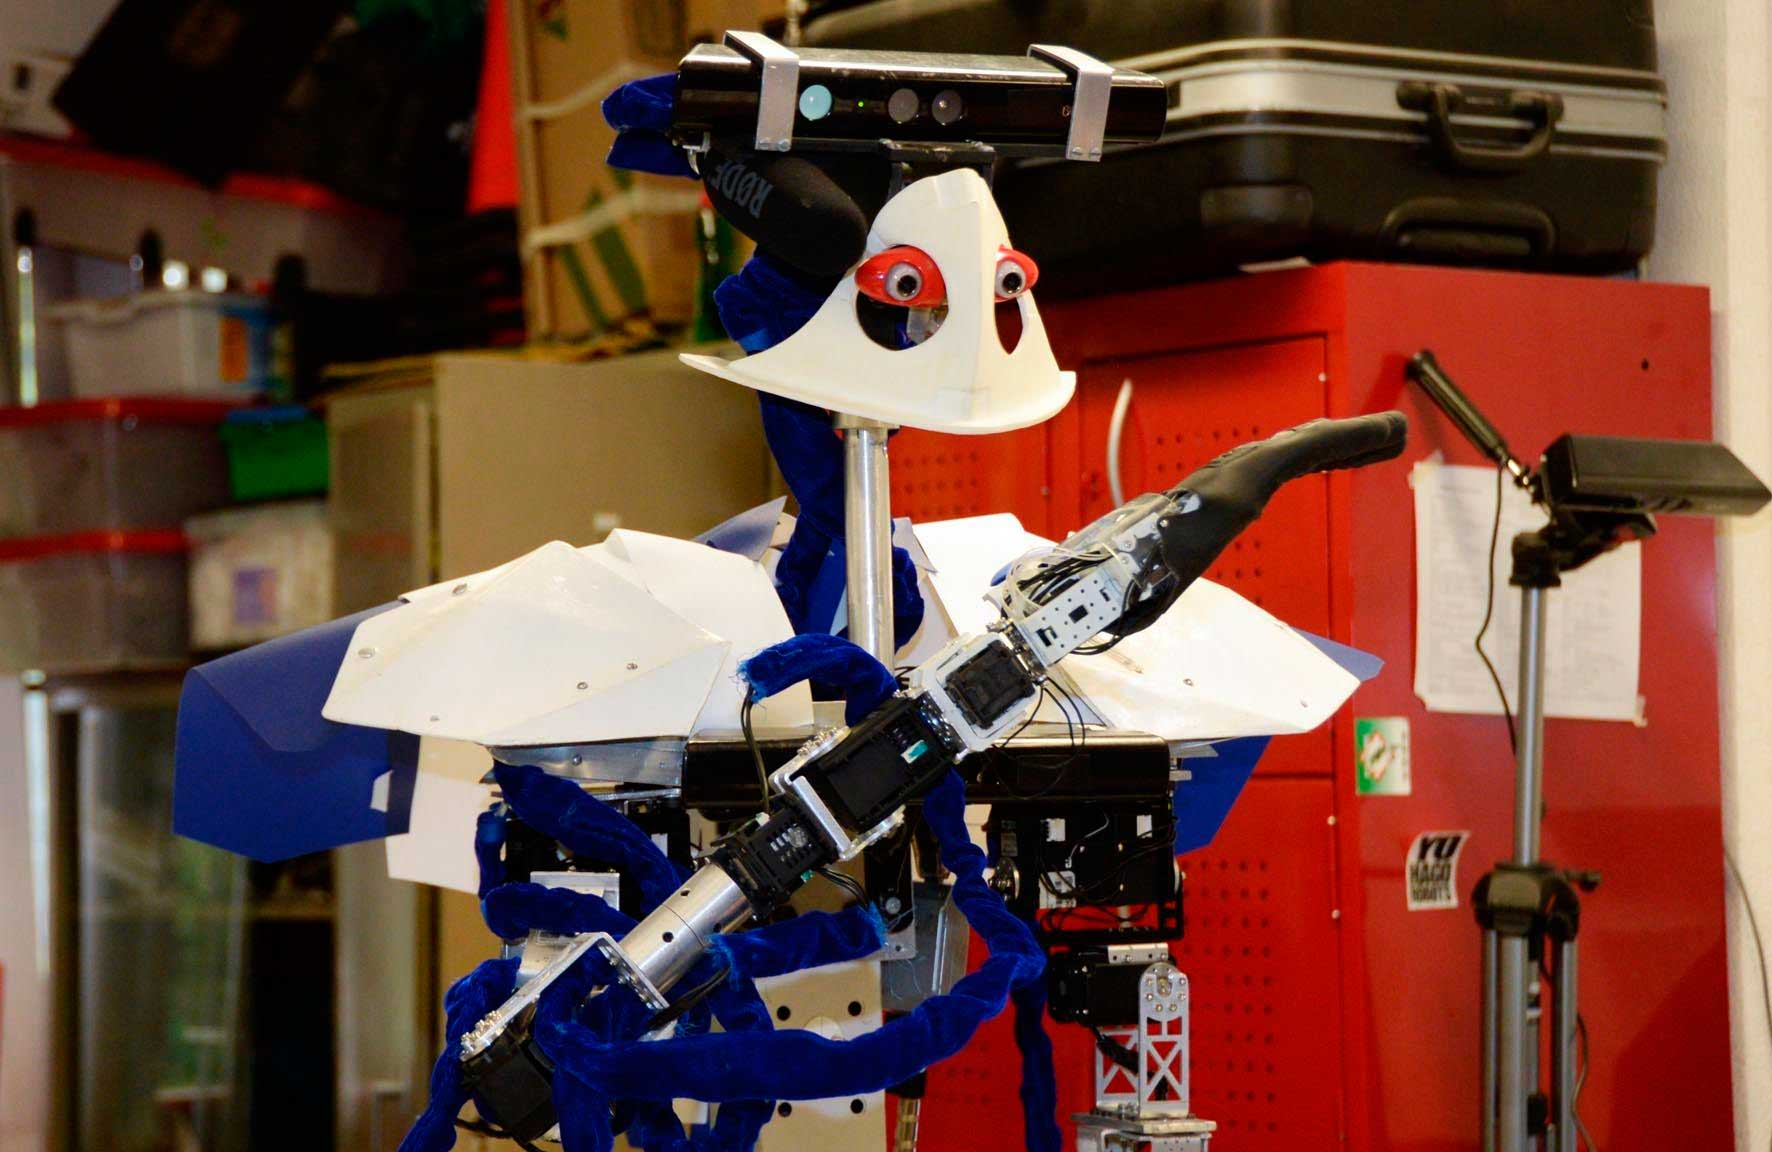
\includegraphics[width=\textwidth]{pumas.jpg}
            \caption{Pumas}
        \end{subfigure} \\
        \begin{subfigure}[b]{.8\linewidth}
            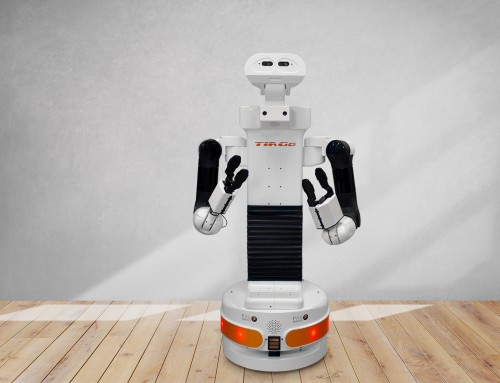
\includegraphics[width=\textwidth]{catie.jpg}
            \caption{CATIE Robotics}
        \end{subfigure} 
    \end{minipage}
    \caption{RoboCup@Home中出现的机器人}
    \label{fig:other_teams}
\end{figure}

\section{本文内容简介}

本章系统的介绍了移动操作机器人的基本定义和国内外研究、应用现状。后续章节将对本文的
主要工作——Tinker移动操作机器人进行介绍,详细的给出Tinker机器人的系统搭建,定位
导航算法的实现与调试,机械臂控制及相应的视觉算法实现以及各部分的版本迭代经过。






% !TeX root = ../main.tex

\chapter{移动操作机器人的系统搭建}
\label{cha:system}


\section{机械结构设计}

按结构划分,可以将Tinker的机械结构粗略的划分为头部,机械臂,骨架,身体主控
以及底盘。机器人的整体外观如图~\ref{fig:tinker_front_side}所示。

\begin{figure}[ht] % use float package if you want it here
  \centering
  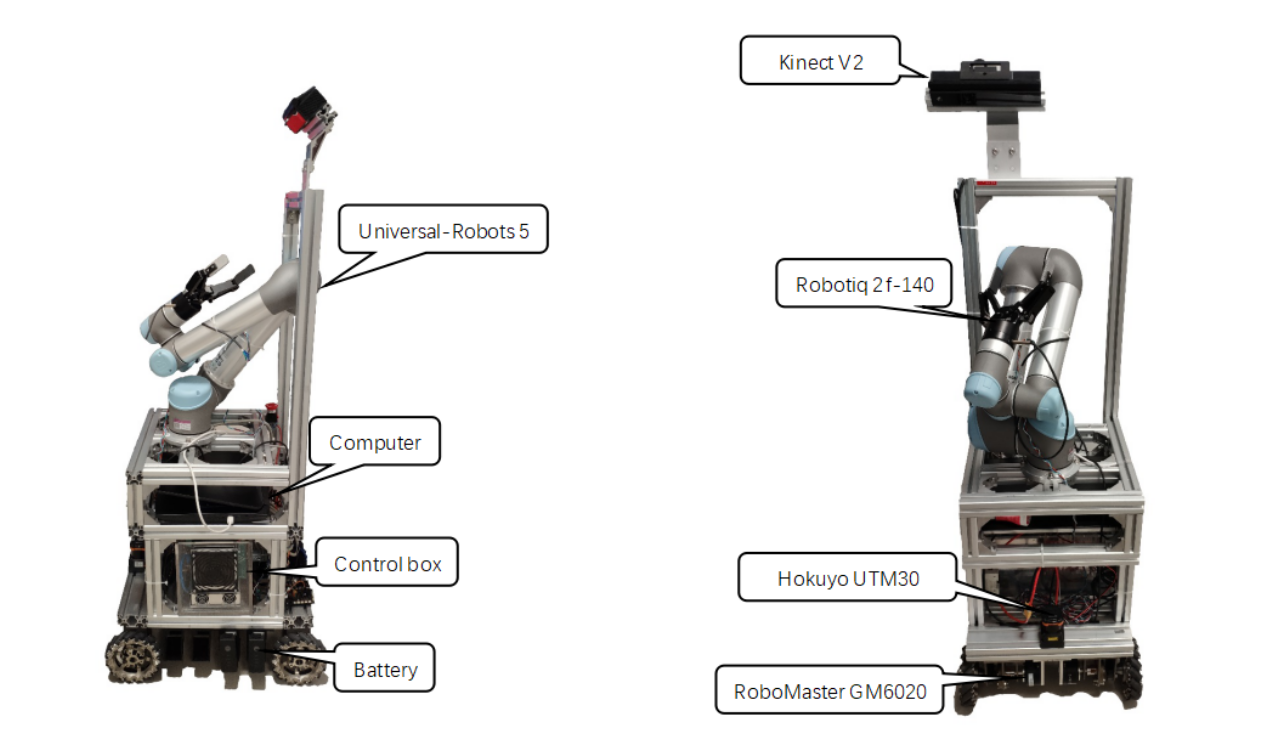
\includegraphics[width=1.\linewidth]{tinker_front_side.png}
  \caption{Tinker前视图与侧视图}
  \label{fig:tinker_front_side}
\end{figure}

\subsection{Tinker骨架搭建}
为方便交通运输与结构迭代,Tinker基本骨架使用40cm*40cm铝形材搭建。骨架
的主要作用为搭建起整个机器人的框架,将各个传感器假设到理想的位置上,并且
为机器人的主控、供电、走线留出足够的空间。经过多轮版本迭代后,目前Tinker
底盘尺寸固定在35cm×45cm,净高140cm,总质量70kg。

为了方便Tinker机器人机械结构长期的维护,降低人员交接成本,我们将Tinker
使用的型材尺寸做了规范化处理,并且对骨架进行了手动建模,以方便机器人的拆
装与改进,如图~\ref{fig:base_link}所示。

\begin{figure}[ht] % use float package if you want it here
  \centering
  \includegraphics[width=.4\linewidth]{base_link.png}
  \caption{Tinker骨架的STL建模结果}
  \label{fig:base_link}
\end{figure}

\subsection{头部设计及版本迭代}

新版的Tinker头部主要用来放置顶部摄像头,在背景环境特别复杂的情况下还会在头部
旁边加装专业的采音麦克风用于语音识别和声源定位。在一般情况下使用头部安装的kinect v2
摄像头自带的麦克风阵列即可满足需求。在Tinker中期我们曾经使用过2自由度云台支持
头部摄像头,使头部摄像头具有上下和左右转动的能力,以扩大摄像头的视野,如图~\ref{fig:neck}
所示。该转台是机器人团队根据现有的通用二自由度转台自行改装的,主要改动有:更换了
原有的舵机,改为精度更高且有位置反馈的dynamixel MX28-AR舵机,
并且相应的改装了转台本身的尺寸和各种装配零件。客观上这一设计确实提高了机器人头部
传感器的视野,但是经过漫长的实践,这一结构被证明是一个彻头彻尾的失败设计。原因有
二:dynamixel本身需要合理的供电和信号线,摄像头本身也有相应的传输线,这些线在频繁
转动的时候很容易被拉断造成整个控制系统崩溃;摄像头本身作为抓取和部分避障的主力
传感器,其位置精度是非常重要的,但是由于舵机空程以及装配过程中产生的空程等等问题,
转台的位置精度一直无法达到要求,大大减弱了摄像头的数据效果。因此在新版的Tinker
中,转台这一设计被机器人团队彻底抛弃了。

\begin{figure}[ht] % use float package if you want it here
  \centering
  \includegraphics[width=.4\linewidth]{neck.png}
  \caption{早期Tinker头部的2自由度转台}
  \label{fig:neck}
\end{figure}

\subsection{Tinker机械臂方案选择}

Tinker使用的机械臂为Universal Robotics公司生产的6自由度机械臂UR5。在决定使用
该机械臂之前我们对市面上在售的各种成品机械臂进行了广泛的调研,包括RoboCup@Home
赛场上使用过的Kinova~\ref{fig:kinova}
机械臂配合三指夹爪,Retinker Robotics公司开发的Sawyer(图~\ref{fig:sawyer})
机械臂,以及Universal Robotics公司出产的各个型号的机械臂(图~\ref{fig:ur_series})。
最终综合考虑了价格、售后、供电、开发者社区等
各个因素后,我们最终确定使用了UR5这个型号的机械臂,并且对机械臂的控制与供电进行了
适当的改装,以符合比赛的需要。

\begin{figure}
\centering
\begin{subfigure}{.5\textwidth}
  \centering
  \includegraphics[width=.9\linewidth]{kinova.png}
  \caption{Kinova}
  \label{fig:kinova}
\end{subfigure}%
\begin{subfigure}{.5\textwidth}
  \centering
  \includegraphics[width=.5\linewidth]{sawyer.jpg}
  \caption{Sawyer}
  \label{fig:sawyer}
\end{subfigure}
\begin{subfigure}{.8\textwidth}
  \centering
  \includegraphics[width=.7\linewidth]{ur_series.jpg}
  \caption{UR系列机械臂}
  \label{fig:ur_series}
\end{subfigure}
\caption{本工作前期调研时关注过得机械臂型号}
\label{fig:arms}
\end{figure}

早期夹爪使用Robotiq
公司生产的Robotiq 2f-85二指夹爪(最大张角85mm),后经过不断的测试与赛场上的较量,
我们发现2f-85的张角对于家庭机器人来说过窄,于是换用了robotiq 2f-140款式的二指夹爪,
该夹爪张角为140mm,能够更好的满足抓取物品、拾取袋子的需求。因此本工作最终使用
UR5 + Robotiq 2f-140作为最终比赛方案,如图~\ref{fig:ur5_2f140}所示。

\begin{figure}[ht] % use float package if you want it here
  \centering
  \includegraphics[width=.4\linewidth]{ur5_2f140.jpeg}
  \caption{Tinker最终使用的机械臂及夹爪方案}
  \label{fig:ur5_2f140}
\end{figure}

\subsection{主控与供电}

Tinker的核心控制由一台搭载了i9-9900K cpu及RTX2080显卡的笔记本电脑完成。在前
几代Tinker设计中,一般主控由工控机或者经过电源改装的台式机担任,但是随着笔记本
性能的不断增强,我们最终选择使用成品机器完成这一任务。成品笔记本性能好,散热完善
且主板设计精良,稳定性好,并且笔记本有自己独立的供电系统,可在机器人断电时单独运行
大大的提升了系统的稳定性和易用性。

整个机器人的供电系统都放在机器人腹部,包括机械臂、底盘、各种传感器、笔记本电脑所需
的所有供电电路以及电池组。2019年Tinker使用单一磷酸铁锂电池供电,标准输出电压29.4V
到24V,容量50AH,放在底盘上部。经过19年比赛的反思之后,作者认为,使用单一锂电池
供电太过危险,且参赛过程中运输太过麻烦,成本过高,于是我们将供电方案改成了多块标准
29V 1500mAH电池并接供电的形式,并3D打印了特制的电池架将电池倒挂在底盘下,这样一方面
大大缩小了Tinker底盘的面积提高了底盘避障导航的灵活性,另一方面降低了整个机器人的中心,
使得机械臂运动时的型变更小,提高了机器人的性能。在供电电路布线方面,Tinker也有了
显著的改进,前一版本中Tinker直接借用了UR5自带的配电箱摆放机械臂及其他部件需要的
供电线路、DCDC、分流排等等元件。但是配电箱本身尺寸过大,不透明,且强度过大,给机器人
装配、调试带来了很大的困难,也对导航的表现造成了影响。之后我们在充分考虑了散热、消防
等等制约之后,使用亚克利版重新制作了一版配电箱,且对机器人的供电线路进行了梳理,大大
缩小了机器人的底盘尺寸,也使得整个供电设计更加简洁易于调试。前后两个版本的供电外观
如图~\ref{fig:elec}所示。

\begin{figure}
\centering
\begin{subfigure}{.5\textwidth}
  \centering
  \includegraphics[height=6cm]{tinker_elec.jpg}
  \caption{改版前的电池及供电线路放置}
  \label{fig:old_elec}
\end{subfigure}%
\begin{subfigure}{.5\textwidth}
  \centering
  \includegraphics[height=6cm]{tinker_elec_new.jpg}
  \caption{改版后的电池及供电线路放置}
  \label{fig:new_elec}
\end{subfigure}
\caption{Tinker前后两个版本的供电布局}
\label{fig:elec}
\end{figure}

\subsection{底盘设计}

Tinker的底盘设计受前几版机器人的影响最多,早期的Tinker使用自制的3自由
度机械臂,其精度有限且自由度受限太严重,需要具有左右额外自由度的底盘
来弥补这一不足,因此Tinker的底盘被设计为使用4个麦克纳母轮的万向底盘
\cite{tlale2008kinematics},底盘设计如图~\ref{fig:chassis_sw}所示,
由于我们使用的麦轮为标准成品,因此在设计图中将麦轮的细节全部简化了。

\begin{figure}[ht] % use float package if you want it here
  \centering
  \includegraphics[width=.7\linewidth]{chassis_sw.png}
  \caption{Tinker底盘悬架的SolidWorks设计图}
  \label{fig:chassis_sw}
\end{figure}

新版Tinker改为成品机械臂后抓取的自由度和覆盖范围都有了质的飞跃,不再要求
底盘具有万向移动的性能了。但是经过多年的改进,机器人团队中对万向底盘的制作
技术已经成熟,于是我们继续沿用了这一设计,仅在电机选型上做了一些与时俱进
的改良,选用了扭矩较大且噪音较小的大疆 GM6020直流无刷电机做底盘的动力电机,
如图~\ref{fig:chassis}所示。

\begin{figure}[ht] % use float package if you want it here
  \centering
  \includegraphics[width=.7\linewidth]{chassis.png}
  \caption{Tinker底盘的电机传动结构}
  \label{fig:chassis}
\end{figure}


\section{电路设计及通信设计}

Tinker机器人作为一个有复杂功能和结构的完整机器人系统,经过长时间的开发
和改进,其控制电路及各个部件之间的通信是及其复杂的。经过不断的实验和试错,
本工作创造性的将软件设计中分定义接口、分层描述的概念引入到机器人
的硬件设计中,对机器人的供电、通信均给出了清晰详尽的分层描述。这一描述大大
的方便了各部分之间的分工协作,提高了开发的效率。

\subsection{供电系统设计及演化}

新版Tinker在搭建之初由于时间紧迫,使用一台逆变器将电池输出的29V直流电源
经过一台逆变器直接转到220V交流电(图~\ref{fig:dc_ac}所示),再连接各个
执行控制部件与传感器。在一段
时间内,这个方案虽然丑陋,但很好的满足了机器人的任务需求,为Tinker机器人的发展
作出了贡献。但是这个方案的缺陷也非常明显,逆变器本身效率很低,且体积不小,
再加上市电转到各个传感器的开销,整个机器人变得异常臃肿,且续航极短。逆变器
工作时还会发出高频啸叫,对机器人的安全和性能都有严重损害。

经过一段时间的调研,作者对Tinker的供电系统做了2次系统的改造,逐步的将
供电改为直流直接供电,并且理顺了机器人内部的供电逻辑。其供电分层描述如图~\ref{fig:charge}
所示

\begin{figure}[ht] % use float package if you want it here
  \centering
  \includegraphics[width=.7\linewidth]{charge.png}
  \caption{Tinker的分层供电示意图}
  \label{fig:charge}
\end{figure}

在供电改造的过程中,最消耗精力的是UR5机械臂的供电改造。UR5机械臂本身所需
的功率极大且其本身的保护机制过于复杂,在机械臂上电时有一套复杂的自检逻辑,
会在直流供电端尝试拉取一个十几A的大电流对电源进行冲击检测,并且在电流拉取
结束后还会反复切断电路进行电源测试。这一逻辑过于复杂,市面上常用的DC-DC
普遍无法满足需求。本文作者经过长时间的反复测试和大量的文献检索,最终
使用明纬SD-1000L-48V开关电源(图~\ref{fig:sd1000l_48}所示)替代普通
电源对机械臂单独供电才满足机械臂的
供电改造需求。

\begin{figure}
\centering
\begin{subfigure}{.5\textwidth}
  \centering
  \includegraphics[width=.6\linewidth]{dc_ac.png}
  \caption{明纬TS-700-248B 700W逆变器}
  \label{fig:dc_ac}
\end{subfigure}%
\begin{subfigure}{.5\textwidth}
  \centering
  \includegraphics[width=.7\linewidth]{sd1000l_48.png}
  \caption{明纬SD-1000L-48V开关电源}
  \label{fig:sd1000l_48}
\end{subfigure}
\caption{Tinker电路改造中使用过的供电元件}
\label{fig:charge_hareware}
\end{figure}

概括的说,Tinker的供电系统中有4个主要电压,分别是电池直接输出且底盘直接
使用的22.2V,机械臂
工作电路需要的48V,笔记本电脑充电需要的19V,各个传感器、路由器以及机械臂
主控需要的12V电压。除机械臂供电使用了明纬SD1000L-48开关电源外,其他变压
需求均使用了一般市售的大功率直流DCDC电源。在经过两轮改版后,Tinker的供电
系统以基本稳定,目前Tinker整机上电待机时长能达到1.5h左右,高负荷运行时(
机械臂高负荷运行且同时执行高强度计算任务,或者底盘不间断运行)可连续工作
20分钟左右,基本满足比赛需求。

\subsection{通信系统设计}

由于Tinker使用了大量的成品部件,包括机械臂、夹爪、电机、各种传感器等等,
其通信设计受限比较大。机器人团队使用开源且在机器人科研领域广泛的ROS框架完成
高层数据及控制通信,辅以必要的底层通信控制,完成整个系统的数据获取与命令
执行功能,其分层设计示意图如~\ref{fig:communication}所示。

\begin{figure}[ht] % use float package if you want it here
  \centering
  \includegraphics[width=.7\linewidth]{communication.png}
  \caption{Tinker的分层通信示意图}
  \label{fig:communication}
\end{figure}

头部Kinect、激光雷达及额外的摄像头(一般安装在机械臂腕部,为一台realsense d435)
通过usb直接连接到中央控制电脑上,通过ros驱动打开,获取的数据流直接发布到
ROS的通信系统中,夹爪使用串口同样连接到电脑上,使用ROS驱动进行控制。UR5
机械臂本身有主控机器,它通过路由器于中央控制电脑连接,两者利用ROS的ethernet
通讯机制通信。麦轮底盘的四个电机统一使用CAN总线连接到一块STM32F4单片机
开发板上,开发板通过PWM控制电机转动,电机内部的编码器数据通过CAN回传到
单片机中,单片机再通过串口与主控电脑通信,为了方便底盘接入Tinker的通信
系统,我们使用rosserial对单片机的串口进行封装,完成控制底盘、获取底盘数据
的功能。


\section{本章小结}

本章详细给出了多模态移动操作机器人Tinker的系统搭建信息,对其结构、供电、电子、
通信、控制原理均给出了详细的设计原理和描述。对关键的部件给出了准确的型号信息,
并且详细的描述了部分结构的迭代信息。

下一章本文将主要讲述移动操作机器人软件开发中的重要技术——移动定位与导航技术,
给出目前定位与导航技术的现状,并且详细描述Tinker机器人的方案选择与方案迭代。










\chapter{移动机器人的定位与导航}
\label{cha:nav}

定位与导航功能在机器人开发中占有重要地位。一般的,我们认为机器人的定位
导航功能包含环境地图构建、路径规划与运动控制以及自主避障等子任务。Tinker
机器人的定位导航系统基于ROS框架下的Navigation Stack实现,使用激光雷达、
里程计、深度相机等多传感器融合方法,能够完成实时地图构建、重定位、动态
环境下的避障及导航任务。


\section{SLAM算法}

SLAM技术(Simultaneous Localization and Mapping)也称为即时定位与地图构建技术,是一种
依赖各种传感器信息获取机器人位姿以及外部地图的技术。SLAM技术对于在机器人行业十分重要,无论是
目前大规模应用的AGV底盘、送餐机器人还是在实验室中被不断开发的各种操作机器人,任何需要移动的
设备都需要SLAM技术进行辅助。按照依赖的主要传感器可以将SLAM技术粗略的划分为两个方向:激光雷达与
视觉方向。SLAM技术近年来发展十分迅速,在多模态融合方向与传统SLAM与深度信息融合方向的发展十分
活跃。下面本文将大致的介绍经典SLAM领域影响交广的研究方向与方法,并给出本文Tinker机器人使用的
SLAM方案和使用心得。

\subsection{SLAM算法现状与原理分析}

在时间上,基于雷达的SLAM算法出现与成熟都比基于视觉的SLAM技术早一些,其原因是多方面的。笔者认为,
一方面是雷达数据,尤其是单线雷达数据,数据量一般比较小,对计算机性能的需求较低,而实时的处理图片
信息对早年的计算机来说的确是相当困难的一件事;另一方面视觉SLAM的许多辅助工具,例如摄像头标定技术,
合适的特征提取算法与最优化工具以及词袋算法,都是相当晚近才完全成熟的,这在一定程度上拖后了视觉SLAM
技术的发展。

\subsubsection{雷达SLAM技术}

最早被广泛接受的雷达SLAM算法应当是Gmapping\cite{grisettiyz2005improving, grisetti2007improved}。
这是一种基于Rao-Blackwellized滤波的粒子滤波算法,它的输入信息为单线激光雷达和里程计,输出为一张2维
地图以及地图原点同里程计坐标原点的位移,这样我们可以根据里程计信息和gmapping给出的地图原点到里程计原点
的坐标差计算出机器人相对于地图的位置。这样算法就一定程度上利用雷达信息消除了里程计的累计误差,提高了定位
的精度(如图~\ref{fig:gmapping},gmapping建出的MIT Killian Court二维地图)

\begin{figure}
  \centering
  \includegraphics[width=300pt]{gmapping.png}
  \caption{Gmapping建出的MIT Killian Court}
  \label{fig:gmapping}
\end{figure}

得益于其不错的性能和便捷易得的开源实现,gmapping算法在机器人领域得到了广泛的应用,尤其是基于ROS的
机器人生态圈中,gmapping有非常重要的地位。但是gmapping算法本身不支持重定位,即一次建图完成之后
下一次运行时读取之前的地图并得到当前机器人相对之前地图位置的能力。这大大的限制了gmapping在应用时
的方便程度。克服这一缺陷的比较常见的方案是使用AMCL\cite{fox2002kld}(这是一种基于蒙特卡罗模拟
的重定位算法)得到新位置相对于老图的位置,然后使用某些微调技术将新图与老图拼接起来。

雷达SLAM领域十分活跃,有相当多使用不同传感器、不同求解方式的算法不断出现,例如使用单线激光雷达与IMU的
Hector SLAM\cite{KohlbrecherMeyerStrykKlingaufFlexibleSlamSystem2011},适用于多线激光雷达
的LOAM\cite{zhang2014loam}等。

近几年最引人注意的成果是google于2016年发布的Cartographer
\cite{hess2016real},同此前的很多雷达定位算法不同,Cartographer的基本求解思想是基于最优化理论的,
这同前文介绍的基于粒子滤波的gmapping有很大不同。Cartographer还引入了Submap的思想,将大的建图场景
分割成相对较小的子图,在局部匹配和全局匹配时都能发挥较好的作用,如图~\ref{fig:cartographer}为
Cartographer的算法框架。Cartographer同时支持2D与3D激光雷达,且
支持多个雷达组合使用以及雷达与IMU的融合,且原生支持地图重定位和分阶段建图,功能十分全面。早期的Cartographer虽然提供ROS的接口,但是其地图格式没有同ROS中主流的Costmap对接起来,随着社区的发展,将Cartographer同ROS
Navigation Stack对接的轮子越来越完善,Cartographer正在快速替代Gmapping成为开源机器人开发者最常
使用的雷达定位算法。如图\ref{fig:cartographer_map}为Cartographer在德国的Deutsches Museum使用
单线激光雷达建图的结果。

\begin{figure}[h] % use float package if you want it here
  \centering
  \includegraphics[width=.95\textwidth]{cartographer.png}
  \caption{Cartographer的算法框架}
  \label{fig:cartographer}
\end{figure}

\begin{figure}
  \centering
  \includegraphics[width=320pt]{cartographer_map.png}
  \caption{Cartographer在Deutsches Museum的建图效果}
  \label{fig:cartographer_map}
\end{figure}



值得一提的,Cartographer中使用的优化框架是Google开发的开源优化器Ceres\cite{ceres-solver},
近几年随着Cartographer等等一些算法的不断出现,Ceres在业内的知名度越来越高,许多基于视觉的SLAM
算法也开始使用Ceres作为优化核心。

\subsubsection{视觉SLAM技术}

视觉SLAM技术的发展更为迅速。从方法上来说可以将视觉SLAM技术笼统的分为直接法、间接法还有半直接法。直接
法是相对于间接法提出的,间接法是指算法在拿到图片后,首先对图片进行特征点提取,然后使用特征点进行后续
的匹配、优化等等过程,因此间接法又被称为特征点法。而直接法是直接使用图片的像素信息进行匹配,一般通过
最小化光度差等等手段进行地图的
重建与位姿提取,而半直接法顾名思意是一种将二者结合的方法。一般直接法对于构建稠密地图有一定优势,但是
专注定位与稀疏建图的算法中还是特征点法占据主流。按照求解思想还可以将视觉SLAM方法划分为使用
优化方法或者滤波方法,目前行业公认优化方法无论在精度、鲁棒性等方面都优于滤波方案。因此本文主要介绍
基于优化的特征点方法中两个具有代表性的算法,以此简要的概括移动操作机器人视觉定位方向的主要形势。

ORB-SLAM算法\cite{mur2015orb}发布时(2015年)在业界引起了很大的震动,这是当时第一款基于特征点
且基本可用的开源单目SLAM算法,在此之前虽然学术界也有一些文章发表,但大多闭源,或者工程实现非常差。
随后一年,原作者又发表并开源了支持双目及RGBD的ORB-SLAM2,ORB-SLAM的影响越来越广泛,可以说这款算法
的发布不但在学术界有极大的影响力,在工业界的震荡也相当大,截止到目前,很多AR企业、基于视觉定位的送餐
机、扫地机等等公司,其核心的定位算法依旧借鉴这款算法开发。ORB-SLAM2算法框架如图~\ref{fig:orb_frame}
所示,在拿到一帧图片后,算法首先对其进行特征提取,特别的这里使用的是ORB特征提取法\cite{rublee2011orb}
,同之前的SIFT、SURF
等等特征提取法不同,ORB算法更适合在CPU上运算,其运算效率比较高,能满足实时性要求。ORB特征点结合了FAST
特征点与Brief描述子,具有方向,且其描述子理论上具有旋转、平移、拉伸不变性,这些特性对于SLAM技术是比较好
的。在完成特征匹配之后,算法会利用描述子将当前帧的特征点与最近的关键帧中的点进行匹配,匹配成功后可以得到
一个粗略
的估计。之后按照一定策略判定当前帧是否是关键帧(例如相邻帧的频率,与上一个关键帧之间的位置差,当前帧的关键
点数等等),如果是的话,要对相关的关键帧再进行一次匹配,以得到可靠的位置约束。在这里ORB-SLAM使用的关键帧
选取策略是共视策略(covisible),即选择在关键帧库中视野与当前帧有交集的那些帧,这种方法相对来说精致一些,
同下文要介绍的VINS有一些不同。上述过程在SLAM领域一般称作Tracking,即追踪过程。为了充分利用环境自带的约束
信息,一般SLAM算法都会在后端运行一个Loop Closing线程,即闭环检测。如图~\ref{fig:loop_closing}所示,
由于累计误差的存在,
在算法运行一段时间视野又回到原点时,其轨迹很可能不会非常理想,但是如果我们能够发现当前的场景和过去的某个
场景有关联,和过去的关键帧建立约束关系,那么此时再对整个轨迹做优化的话,就能很好的消除累计误差,得到不错的
定位效果。ORB SLAM中寻找相似场景主要依赖BoW(Bag of Words,词袋)技术\cite{GalvezTRO12}。基于特征点
与关键帧的ORB-SLAM算法可视化效果如图~\ref{fig:orb_viz}所示,目前大多数基于特征点的SLAM算法都使用
关键帧作为管理点的单位,因此很多算法的可视化效果都和此图差不多。


\begin{figure}[h] % use float package if you want it here
  \centering
  \includegraphics[width=.95\textwidth]{loop_closing.png}
  \caption{应用闭环约束前后的轨迹变化}
  \label{fig:loop_closing}
\end{figure}


\begin{figure}[h] % use float package if you want it here
  \centering
  \includegraphics[width=300pt]{orb_viz.jpg}
  \caption{ORB-SLAM运行时的可视化效果}
  \label{fig:orb_viz}
\end{figure}

\begin{figure}[h] % use float package if you want it here
  \centering
  \includegraphics[width=.95\textwidth]{orb_framework.png}
  \caption{ORB-SLAM2的算法框架}
  \label{fig:orb_frame}
\end{figure}




VINS\cite{qin2018vins}算法大致比ORB-SLAM晚2-3年出现,诞生于香港科技大学Shaojie Shen团队,VINS-Mono的发表时间是2018年,VINS-Fusion
稍晚一些,它也是基于优化方案的特征点法SLAM
算法。同ORB-SLAM不同的是,VINS给出了视觉与IMU融合的有效解决方案,有了IMU的辅助VINS在表现上
更加鲁棒,精度也更高,尤其在无人机定位方向表现非常出彩。VINS对IMU数据的一项重要处理手段是IMU预积分
技术(IMU preintegratio),一般认为,这项技术的最早提出是佐治亚理工的C. Foster于2015年发表的
\cite{forster2015imu},而沈的团队于15年发表的\cite{shen2015tightly}就详细的分析了将IMU预积分
应用到无人机的视觉定位算法中的可能性,这篇文章可以视作是VINS的准备工作。如图~\ref{fig:vins_frame}
展示了VINS的算法框架,可以看到VINS的大致工作流程同ORB-SLAM是差不太多的,但是在某些算法方案上有不同。
例如VINS的关键帧选取策略与ORB-SLAM的共视不同,是简单的Sliding Windows方案,即不管当前帧位姿如何
算法都选取临近的若干帧进行位姿优化。这种方案有一定的道理:首先相机是均匀连续移动的这一假设在大多数情况下
都应当是成立的;其次,有IMU数据的修正,算法理论上更加不容易失配,选择相对简单的策略也就是被允许的了。


\begin{figure}[h] % use float package if you want it here
  \centering
  \includegraphics[width=.95\textwidth]{vins_framework.png}
  \caption{VINS-Mono的算法框架}
  \label{fig:vins_frame}
\end{figure}

\subsection{SLAM算法选择与性能分析}


Tinker最初使用的是建图与定位分开实现的方案。建图方面,我们使用
gmapping算法\cite{grisettiyz2005improving},
依赖2个北洋UTM-30LX单线激光雷达拼接定位(如图~\ref{fig:utm30lx})。定位
方面,我们使用基于蒙特卡罗的
amcl算法\cite{fox2002kld},两个算法同时工作时的可视化信息如图~\ref{fig:gmapping_amcl}。
amcl需要在地图已经给出的情况下进行定位,在
真实赛场上,比赛场景多数情况下是确定的,因此这套方案还基本可用,Tinker机器人
会在开赛前对赛场进行扫描,将地图场景保存起来,之后比赛过程中单纯使用amcl
进行定位。后期随着团队成员对这套定位算法越来越熟悉,我们会将场景内可能出现
在单线雷达视野内的一切固定障碍的尺寸量下来,使用绘图软件对地图进行重建,然后
使用amcl进行定位,可以拿到更好的定位效果。

\begin{figure}
  \centering
  \includegraphics[width=150pt]{utm30lx.jpeg}
  \caption{北洋UTM-30LX单线激光雷达}
  \label{fig:utm30lx}
\end{figure}


\begin{figure}
  \centering
  \includegraphics[width=300pt]{gmapping_amcl.png}
  \caption{Gmapping + Amcl可视化效果}
  \label{fig:gmapping_amcl}
\end{figure}

虽然上述方案在长时间内被证明是稳定可用的,但随着SLAM社区的不断发展,基于
粒子滤波的定位建图算法已经过时了,尤其是Google开源其自主开发的Cartographer
雷达建图定位算法\cite{hess2016real}之后,本工作后期也将定位方案迁移为Cartographer+
ROS Navigation的模式,在更换建图定位算法之后,配合我们对Tinker硬件的二次
改版,我们也将原有的2个单线雷达减少为一个,变动之后定位数据减少,运算效率也
得到了提升。Cartographer的算法框架如图~\ref{fig:cartographer}所示。


除了基于单线激光雷达的各种定位建图算法外,笔者还尝试了一些基于特征点的视觉SLAM
方案,例如基于ORB特征点法的ORB-SLAM2(使用Kinect v2的RGB-D数据)\cite{mur2015orb},
ORB-SLAM2在室内环境中的可视化效果如图TODO所示。我们还测试了基于双目和IMU数据
融合的VINS-Fusion\cite{qin2018vins}算法,并且分析了两算法表现上的差异。

ORB-SLAM2的算法框架如图~\ref{fig:orb_frame}所示,其获取到原始数据后,首先对左右
目的图像提取特征,完成三角化,之后使用特征点的描述子在关键帧库中选取合适的帧
进行匹配,ORB-SLAM的关键帧选取策略较复杂,是一种基于共视关系的选取方案,即我们
在仓库中选取可能和当前帧看到同一场景的帧来进行匹配,在完成局部位姿优化后,经过
关键帧筛选策略选取关键帧,之后后端不断尝试通过词袋法发现相同场景,完成大的闭环
优化。VINS的算法框架如图~\ref{fig:vins_frame}所示,vins也是基于关键点法进行位姿
匹配的算法,同ORB-SLAM的主要区别有两个:一是VINS有IMU融合,其处理IMU数据的方式
为IMU预积分(IMU preintegration)\cite{forster2015manifold},且它将处理结果作为
优化项中的一个因子参与了位姿优化;二是VINS的
关键帧选择策略是简单的Sliding Window算法,即选取与当前帧在时间上相邻的几个关键帧
进行特征匹配与优化,这个策略和ORB-SLAM的共视图策略想比较略显粗糙,但是在大场景
下还是有不错的匹配效果。




\section{导航方案的选择}

Tinker的开发过程中一直使用ROS作为主要开发框架,而ROS的Navigation Stack中对于
导航避障提供了一套较为成熟的解决方案。Tinker前后使用了2套定位与规划算法,下面两个
章节中将对这两套方案进行详细描述。

\subsection{路径规划}

ROS的Navigation stack中提供了一整套导航避障的解决方案。其核心是同时维护地图信息
与路径规划器。地图信息使用一种分层管理的方式\cite{lu2014layered},并且分别维护
全局地图 Global Map与局部地图 Local Map。规划器也有两个,分别是Global Planner
和Local Planner。其中 Global Planner负责根据全局地图生成路径,而 Local Planner
则负责根据局部地图生成速度指令,传输给底盘执行。Tinker使用的 Global Planner是
一种基于 Dijkstra算法\cite{deng2012fuzzy}的路径生成方法,Local Planner是
一种基于dynamic window approach的速度生成方案\cite{fox1997dynamic}如图,其算法思想
为:在当前位置向各个方向以不同速度发射模拟路径,并且按照这些路径是否经过障碍物、
离目标路径的远近等等条件本别进行打分,选取分数最高的路径对应的速度极为dwa的输出
结果~\ref{fig:dwa}。上述
方案均为机器人导航领域较为经典且通用的方案,本工作对上述算法进行了一些微调,以
使算法在Tinker平台上有更好的表现,如图~\ref{nav_costmap}所示为Tinker进行导航任
务时可视化的调试信息。


\begin{figure}[h] % use float package if you want it here
  \centering
  \includegraphics[width=1.\textwidth]{dwa.png}
  \caption{dwa算法示意图}
  \label{fig:dwa}
\end{figure}


\begin{figure}[h] % use float package if you want it here
  \centering
  \includegraphics[width=1.\textwidth]{nav_costmap.png}
  \caption{进行导航任务时的地图与路径}
  \label{fig:nav_costmap}
\end{figure}

\subsection{机器人控制}

由于Tinker机器人使用全向麦克纳姆轮底盘,且每个电机控制一个麦轮,其运动学解算同
传统2轮底盘或者4轮阿克曼转向底盘相比更复杂一些。


\begin{figure}[h] % use float package if you want it here
  \centering
  \includegraphics[width=.95\textwidth]{mecanum.png}
  \caption{麦轮底盘(左)与麦轮放大图(右),图片来源\cite{mecanum}}
  \label{fig:mecanum}
\end{figure}

如图~\ref{fig:mecanum}所示,假设底盘麦轮X型安装,其4轮到底盘中心的横向纵向距离分别
为$L_1$、$L_2$,四个车轮的转速为$\omega_1$、$\omega_2$、$\omega_3$、$\omega_4$
(即为电机转速),四个车轮上滚子的速度分别为$v_{g1}$、$v_{g2}$、$v_{g3}$、$v_{g4}$,
四个轮子的主轴的瞬时速度为$v_{O1x}, v_{O1y}$,$v_{O2x}, v_{O2y}$,$v_{O3x}, v_{O3y}$,
$v_{O4x}, v_{O4y}$,整个底盘的速度可表示为$v_x, v_y, \omega_O$,麦轮滚子轴与麦轮主轴
的夹角为$\alpha$(一般为\ang{45}),麦轮滚子轴到主轴的距离为$R$

根据速度分解,对1轮可列出~\ref{equ:glo_vec};对单个麦轮进行速度分析,可得~\ref{equ:loc_vec}

\begin{equation}
  \label{equ:glo_vec}
  \begin{aligned}
    v_{O1x} = v_x - \omega_O * L_1\\
    v_{O1y} = v_y - \omega_O * L_2
  \end{aligned}
\end{equation}

\begin{equation}
  \label{equ:loc_vec}
  \begin{aligned}
    v_{O1x} &= - v_{g1} * \cos\alpha + \omega_1 * R\\
    v_{O1y} &= v_{g1} * \sin\alpha
  \end{aligned}
\end{equation}

将~\ref{equ:glo_vec}~\ref{equ:loc_vec}两式联立消去轮速,可得~\ref{equ:mid_equ},
将两式合并消去$v_{g1}$,最终得到~\ref{equ:fin_equ}。

\begin{equation}
  \label{equ:mid_equ}
  \begin{aligned}
    v_x - \omega_O * L_1 &= - v_{g1} * \cos\alpha + \omega_1 * R \\
    v_y - \omega_O * L_2 &= v_{g1} * \sin\alpha
  \end{aligned}
\end{equation}


\begin{equation}
  \label{equ:fin_equ}
  \omega_1 = \frac{1}{R}
    \begin{bmatrix}
      1 & \frac{1}{\tan\alpha} & -(L_1 + \frac{L_2}{\tan\alpha})
    \end{bmatrix}
    \begin{bmatrix}
      v_x \\
      v_y \\
      \omega_O
    \end{bmatrix}
\end{equation}

因为此处$\alpha$取值为\ang{45},将其带入后可以得到四个轮子的电机输出转速与目标速度的转换
公式为\ref{equ:fin_all}

\begin{equation}
  \label{equ:fin_all}
  \begin{bmatrix}
    \omega_1 \\
    \omega_2 \\
    \omega_3 \\
    \omega_4
  \end{bmatrix}
    = \frac{1}{R}
  \begin{bmatrix}
    1 &  1 & -(L_1 + L_2) \\
    1 & -1 &  (L_1 + L_2) \\
    1 & -1 & -(L_1 + L_2) \\
    1 &  1 &  (L_1 + L_2) \\
  \end{bmatrix}
  \begin{bmatrix}
    v_x \\
    v_y \\
    \omega_O
  \end{bmatrix}
\end{equation}

值得一提的是通过不断探索,作者发现:在底盘接受速度命令端加一个smoother,对临近的
几帧速度命令进行一定程度的加权平滑(即一个一阶低通滤波器)~\ref{equ:filter}能够使
机器人的运动性能得到质的提升,本文使用的一阶低通滤波算法如下:

\begin{equation}
  \label{equ:filter}
  v_{final} = 0.9 * v_{origin} + 0.1 * v_{cur}
\end{equation}

这一发现也提示我们,对于机器人这一复杂系统来说,提升整体性能的手段是多元的,在制
定方案时应勇于尝试
多做实验,积极尝试各种想法,这样有助于我们使用较低的成本达到更好的性能。

\section{本章小结}

本章较为概括的描述了机器人定位导航领域的大致现状,并且选取了领域内具有划时代意义且目前依然
使用广泛的几个算法进行重点介绍;同时,本章完整的给出了Tinker机器人移动定位导航方向使用的
方案以及开发过程中的经验教训。

下一章,本文将介绍移动操作机器人的重点技术——视觉检测与机械臂规划。







%%% 其它部分
\backmatter

%% 本科生要这几个索引,研究生不要。选择性留下。
% 插图索引
%\listoffigures
% 表格索引
%\listoftables
% 公式索引
%\listofequations


%% 参考文献
% 只能选择一种参考文献格式
\bibliographystyle{thuthesis-numeric}      % 顺序编码制
% \bibliographystyle{thuthesis-author-year}  % 著者-出版年制
% \bibliographystyle{thuthesis-bachelor}     % 本科生参考文献的著录格式
\bibliography{ref/refs}


%% 致谢
%\input{data/ack}

%% 附录
%\begin{appendix}
%\input{data/appendix01}
%\end{appendix}

%% 个人简历
%\input{data/resume}

%% 本科生进行格式审查是需要下面这个表格,答辩可能不需要。选择性留下。
% 综合论文训练记录表
%\includepdf[pages=-]{scan-record.pdf}
\end{document}
